        %%******************************************%%
        %%                                          %%
        %%        Modello di tesi di laurea         %%
        %%            di Andrea Giraldin            %%
        %%                                          %%
        %%             2 novembre 2012              %%
        %%                                          %%
        %%******************************************%%


% I seguenti commenti speciali impostano:
% 1. 
% 2. PDFLaTeX come motore di composizione;
% 3. tesi.tex come documento principale;
% 4. il controllo ortografico italiano per l'editor.

% !TEX encoding = UTF-8
% !TEX TS-program = pdflatex
% !TEX root = tesi.tex
% !TEX spellcheck = it-IT

% PDF/A filecontents
\RequirePackage{filecontents}
\begin{filecontents*}{\jobname.xmpdata}
  \Title{Document’s title}
  \Author{Author’s name}
  \Language{it-IT}
  \Subject{The abstract, or short description.}
  \Keywords{keyword1\sep keyword2\sep keyword3}
\end{filecontents*}

\documentclass[10pt,                    % corpo del font principale
               a4paper,                 % carta A4
              % twoside,                 % impagina per fronte-retro
               openright,               % inizio capitoli a destra
               english,                 
               italian,  
               openany               
               ]{book}    

%**************************************************************
% Importazione package
%************************************************************** 

\PassOptionsToPackage{dvipsnames}{xcolor} % colori PDF/A

\usepackage{colorprofiles}

\usepackage[a-2b,mathxmp]{pdfx}[2018/12/22]
                                        % configurazione PDF/A
                                        % validare in https://www.pdf-online.com/osa/validate.aspx

%\usepackage{amsmath,amssymb,amsthm}    % matematica

\usepackage[T1]{fontenc}                % codifica dei font:
                                        % NOTA BENE! richiede una distribuzione *completa* di LaTeX

\usepackage[utf8]{inputenc}             % codifica di input; anche [latin1] va bene
                                        % NOTA BENE! va accordata con le preferenze dell'editor

\usepackage[english, italian]{babel}    % per scrivere in italiano e in inglese;
                                        % l'ultima lingua (l'italiano) risulta predefinita

\usepackage{bookmark}                   % segnalibri

\usepackage{caption}                    % didascalie

\usepackage{chngpage,calc}              % centra il frontespizio

\usepackage{csquotes}                   % gestisce automaticamente i caratteri (")

\usepackage{emptypage}                  % pagine vuote senza testatina e piede di pagina

\usepackage{epigraph}			% per epigrafi

\usepackage{eurosym}                    % simbolo dell'euro

%\usepackage{indentfirst}               % rientra il primo paragrafo di ogni sezione

\usepackage{graphicx}                   % immagini

\usepackage{hyperref}                   % collegamenti ipertestuali

\usepackage[binding=5mm]{layaureo}      % margini ottimizzati per l'A4; rilegatura di 5 mm

\usepackage{listings}                   % codici

\usepackage{microtype}                  % microtipografia

\usepackage{mparhack,fixltx2e,relsize}  % finezze tipografiche

\usepackage{nameref}                    % visualizza nome dei riferimenti                                      
\usepackage[font=small]{quoting}        % citazioni

\usepackage{subfig}                     % sottofigure, sottotabelle

\usepackage[italian]{varioref}          % riferimenti completi della pagina

\usepackage{booktabs}                   % tabelle                                       
\usepackage{tabularx}                   % tabelle di larghezza prefissata                                    
\usepackage{longtable}                  % tabelle su più pagine                                        
\usepackage{ltxtable}                   % tabelle su più pagine e adattabili in larghezza

\usepackage[toc, acronym]{glossaries}   % glossario
                                        % per includerlo nel documento bisogna:
                                        % 1. compilare una prima volta tesi.tex;
                                        % 2. eseguire: makeindex -s tesi.ist -t tesi.glg -o tesi.gls tesi.glo
                                        % 3. eseguire: makeindex -s tesi.ist -t tesi.alg -o tesi.acr tesi.acn
                                        % 4. compilare due volte tesi.tex.

\usepackage[backend=biber,style=verbose-ibid,hyperref,backref]{biblatex}
                                        % eccellente pacchetto per la bibliografia; 
                                        % produce uno stile di citazione autore-anno; 
                                        % lo stile "numeric-comp" produce riferimenti numerici
                                        % per includerlo nel documento bisogna:
                                        % 1. compilare una prima volta tesi.tex;
                                        % 2. eseguire: biber tesi
                                        % 3. compilare ancora tesi.tex.

%**************************************************************
% file contenente le impostazioni della tesi
%**************************************************************

%**************************************************************
% Frontespizio
%**************************************************************

% Autore
\newcommand{\myName}{Lorenzo Brescanzin}                                    
\newcommand{\myTitle}{Titolo della tesi}

% Tipo di tesi                   
\newcommand{\myDegree}{Tesi di laurea}

% Università             
\newcommand{\myUni}{Università degli Studi di Padova}

% Facoltà       
\newcommand{\myFaculty}{Corso di Laurea in Informatica}

% Dipartimento
\newcommand{\myDepartment}{Dipartimento di Matematica "Tullio Levi-Civita"}

% Titolo del relatore
\newcommand{\profTitle}{Prof.}

% Relatore
\newcommand{\myProf}{Tullio Vardanega}

% Luogo
\newcommand{\myLocation}{Padova}

% Anno accademico
\newcommand{\myAA}{2020-2021}

% Data discussione
\newcommand{\myTime}{Dicembre 2021}


%**************************************************************
% Impostazioni di impaginazione
% see: http://wwwcdf.pd.infn.it/AppuntiLinux/a2547.htm
%**************************************************************

\setlength{\parindent}{14pt}   % larghezza rientro della prima riga
\setlength{\parskip}{0pt}   % distanza tra i paragrafi


%**************************************************************
% Impostazioni di biblatex
%**************************************************************
\bibliography{bibliografia} % database di biblatex 

\defbibheading{bibliography} {
    \cleardoublepage
    \phantomsection 
    \addcontentsline{toc}{chapter}{\bibname}
    \chapter*{\bibname\markboth{\bibname}{\bibname}}
}

\setlength\bibitemsep{1.5\itemsep} % spazio tra entry

\DeclareBibliographyCategory{opere}
\DeclareBibliographyCategory{web}

\addtocategory{opere}{womak:lean-thinking}
\addtocategory{web}{site:agile-manifesto}

\defbibheading{opere}{\section*{Riferimenti bibliografici}}
\defbibheading{web}{\section*{Siti Web consultati}}


%**************************************************************
% Impostazioni di caption
%**************************************************************
\captionsetup{
    tableposition=top,
    figureposition=bottom,
    font=small,
    format=hang,
    labelfont=bf
}

%**************************************************************
% Impostazioni di glossaries
%**************************************************************

%**************************************************************
% Acronimi
%**************************************************************
\renewcommand{\acronymname}{Acronimi e abbreviazioni}

\newacronym[description={\glslink{aws}{Amazon Web Services}}]
    {aws}{AWS}{Amazon Web Services}

\newacronym[description={\glslink{apig}{Application Program Interface}}]
    {api}{API}{Application Program Interface}

\newacronym[description={Model-View-ViewModel}]
    {mvvm}{MVVM}{Model-View-ViewModel}

\newacronym[description={Internet of Things}]
    {iot}{IoT}{Internet of Things}

\newacronym[description={Database Management System}]
    {dbms}{DBMS}{Database Management System}

\newacronym[description={JavaScript Obbject Notation}]
    {json}{JSON}{JavaScript Obbject Notation}

\newacronym[description={Test-Driven Development}]
    {tdd}{TDD}{Test-Driven Development}

\newacronym[description={Information Technology}]
    {it}{IT}{Information Technology}

\newacronym[description={Unified Model Language}]
    {uml}{UML}{Unified Model Language}

\newacronym[description={Representational State Transfer}]
    {rest}{REST}{Representational State Transfer}

\newacronym[description={Electronic Data Interchange}]
    {edi}{EDI}{Electronic Data Intechange}

\newacronym[description={HyperText Transfer Protocol}]
    {http}{HTTP}{HyperText Transfer Protocol}

\newacronym[description={Entity-Relationship}]
    {er}{ER}{Entity-Relationship}   

\newacronym[description={DataBase Markup Language}]
    {dbml}{DBML}{DataBase Markup Language}

\newacronym[description={Inversion of Control}]
    {ioc}{IoC}{Inversion of Control} 
    
\newacronym[description={User Interfaces}]
    {ui}{UI}{User Interface}

\newacronym[description={Model-View-Controller}]
    {mvc}{MVC}{Model-View-Controller}

\newacronym[description={Integrated Development Environment}]
    {ide}{IDE}{Integrated Development Environment}
%**************************************************************
% Glossario
%**************************************************************
%\renewcommand{\glossaryname}{Glossario}

\newglossaryentry{apig}
{
    name=\glslink{api}{API},
    text=Application Program Interface,
    sort=api,
    description={in informatica con il termine \emph{\acrfull{api}} si indica ogni insieme di procedure disponibili al programmatore, di solito raggruppate a formare un set di strumenti specifici per l'espletamento di un determinato compito all'interno di un certo programma. La finalità è ottenere un'astrazione, di solito tra l'hardware e il programmatore o tra software a basso e quello ad alto livello semplificando così il lavoro di programmazione}
}

%\newglossaryentry{umlg}
%{
%    name=\glslink{uml}{UML},
%    text=UML,
%    sort=uml,
%    description={in ingegneria del software \emph{UML, Unified Modeling Language} (ing. linguaggio di modellazione unificato) è un linguaggio di modellazione e specifica basato sul paradigma object-oriented. L'\emph{UML} svolge un'importantissima funzione di ``lingua franca'' nella comunità della progettazione e programmazione a oggetti. Gran parte della letteratura di settore usa tale linguaggio per descrivere soluzioni analitiche e progettuali in modo sintetico e comprensibile a un vasto pubblico}
%}

\newglossaryentry{mock-up}
{
    name=Mock-Up,
    text=mock-up,
    sort=mock-up,
    description={Durante la progettazione un \emph{mock-up} è un modello utilizzato, ad esempio, per valutare la bontà della progettazione effettuata o per ottenere dei \emph{feedbacks} da parte dei clienti}
}

\newglossaryentry{backend}
{
    name=Backend,
    text=backend,
    sort=backend,
    description={Un'applicazione backend è un programma con il quale l'utente interagisce indirettamente, in generale attraverso l'utilizzo di un'applicazione \gls{frontend}. In una struttura client/server il backend è il server}
}

\newglossaryentry{open-source}
{
    name=Open-Source,
    text=open-source,
    sort=open-source,
    description={Per \emph{software open-source} si intende \emph{software} il cui codice sorgente è disponibile al pubblico, il quale può visionarlo e modificarlo. Il modello \emph{open-source} è un modello di sviluppo decentralizzato che incoraggia la collaborazione}
}

\newglossaryentry{frontend}
{
    name=Frontend,
    text=frontend,
    sort=frontend,
    description={Un'applicazione frontend è un programma con il quale l'utente interagisce direttamente. In una struttura client/server il frontend è il client.}
}

\newglossaryentry{stakeholder}
{
    name=Stakeholder,
    text=stakeholder,
    sort=stakeholder,
    description={Portatori di interesse. Nell'ambito del software, possono essere i clienti, fornitori, finanziatori e banche.}
}
 % database di termini
\makeglossaries


%**************************************************************
% Impostazioni di graphicx
%**************************************************************
\graphicspath{{immagini/}} % cartella dove sono riposte le immagini


%**************************************************************
% Impostazioni di hyperref
%**************************************************************
\hypersetup{
    %hyperfootnotes=false,
    %pdfpagelabels,
    %draft,	% = elimina tutti i link (utile per stampe in bianco e nero)
    colorlinks=true,
    linktocpage=true,
    pdfstartpage=1,
    pdfstartview=,
    % decommenta la riga seguente per avere link in nero (per esempio per la stampa in bianco e nero)
    %colorlinks=false, linktocpage=false, pdfborder={0 0 0}, pdfstartpage=1, pdfstartview=FitV,
    breaklinks=true,
    pdfpagemode=UseNone,
    pageanchor=true,
    pdfpagemode=UseOutlines,
    plainpages=false,
    bookmarksnumbered,
    bookmarksopen=true,
    bookmarksopenlevel=1,
    hypertexnames=true,
    pdfhighlight=/O,
    %nesting=true,
    %frenchlinks,
    urlcolor=webbrown,
    linkcolor=RoyalBlue,
    citecolor=webgreen,
    %pagecolor=RoyalBlue,
    %urlcolor=Black, linkcolor=Black, citecolor=Black, %pagecolor=Black,
    pdftitle={\myTitle},
    pdfauthor={\textcopyright\ \myName, \myUni, \myFaculty},
    pdfsubject={},
    pdfkeywords={},
    pdfcreator={pdfLaTeX},
    pdfproducer={LaTeX}
}

%**************************************************************
% Impostazioni di itemize
%**************************************************************
%\renewcommand{\labelitemi}{$\ast$}
\renewcommand{\labelitemi}{$\bullet$}
%\renewcommand{\labelitemii}{$\cdot$}
%\renewcommand{\labelitemiii}{$\diamond$}
%\renewcommand{\labelitemiv}{$\ast$}


%**************************************************************
% Impostazioni di listings
%**************************************************************
\lstset{
    language=[LaTeX]Tex,%C++,
    keywordstyle=\color{RoyalBlue}, %\bfseries,
    basicstyle=\small\ttfamily,
    %identifierstyle=\color{NavyBlue},
    commentstyle=\color{Green}\ttfamily,
    stringstyle=\rmfamily,
    numbers=none, %left,%
    numberstyle=\scriptsize, %\tiny
    stepnumber=5,
    numbersep=8pt,
    showstringspaces=false,
    breaklines=true,
    frameround=ftff,
    frame=single
} 


%**************************************************************
% Impostazioni di xcolor
%**************************************************************
\definecolor{webgreen}{rgb}{0,.5,0}
\definecolor{webbrown}{rgb}{.6,0,0}


%**************************************************************
% Altro
%**************************************************************

\newcommand{\omissis}{[\dots\negthinspace]} % produce [...]

% eccezioni all'algoritmo di sillabazione
\hyphenation
{
    ma-cro-istru-zio-ne
    gi-ral-din
}

\newcommand{\sectionname}{sezione}
\addto\captionsitalian{\renewcommand{\figurename}{Figura}
                       \renewcommand{\tablename}{Tabella}}

\newcommand{\glsfirstoccur}{\ap{{[g]}}}

\newcommand{\intro}[1]{\emph{\textsf{#1}}}

%**************************************************************
% Environment per ``rischi''
%**************************************************************
\newcounter{riskcounter}                % define a counter
\setcounter{riskcounter}{0}             % set the counter to some initial value

%%%% Parameters
% #1: Title
\newenvironment{risk}[1]{
    \refstepcounter{riskcounter}        % increment counter
    \par \noindent                      % start new paragraph
    \textbf{\arabic{riskcounter}. #1}   % display the title before the 
                                        % content of the environment is displayed 
}{
    \par\medskip
}

\newcommand{\riskname}{Rischio}

\newcommand{\riskdescription}[1]{\textbf{\\Descrizione:} #1.}

\newcommand{\risksolution}[1]{\textbf{\\Soluzione:} #1.}

%**************************************************************
% Environment per ``use case''
%**************************************************************
\newcounter{usecasecounter}             % define a counter
\setcounter{usecasecounter}{0}          % set the counter to some initial value

%%%% Parameters
% #1: ID
% #2: Nome
\newenvironment{usecase}[2]{
    \renewcommand{\theusecasecounter}{\usecasename #1}  % this is where the display of 
                                                        % the counter is overwritten/modified
    \refstepcounter{usecasecounter}             % increment counter
    \vspace{10pt}
    \par \noindent                              % start new paragraph
    {\large \textbf{\usecasename #1: #2}}       % display the title before the 
                                                % content of the environment is displayed 
    \medskip
}{
    \medskip
}

\newcommand{\usecasename}{UC}

\newcommand{\usecaseactors}[1]{\textbf{\\Attori Principali:} #1. \vspace{4pt}}
\newcommand{\usecasepre}[1]{\textbf{\\Precondizioni:} #1. \vspace{4pt}}
\newcommand{\usecasedesc}[1]{\textbf{\\Descrizione:} #1. \vspace{4pt}}
\newcommand{\usecasepost}[1]{\textbf{\\Postcondizioni:} #1. \vspace{4pt}}
\newcommand{\usecasealt}[1]{\textbf{\\Scenario Alternativo:} #1. \vspace{4pt}}

%**************************************************************
% Environment per ``namespace description''
%**************************************************************

\newenvironment{namespacedesc}{
    \vspace{10pt}
    \par \noindent                              % start new paragraph
    \begin{description} 
}{
    \end{description}
    \medskip
}

\newcommand{\classdesc}[2]{\item[\textbf{#1:}] #2}
                     % file con le impostazioni personali

\begin{document}
%**************************************************************
% Materiale iniziale
%**************************************************************
\frontmatter
\input{inizio-fine/frontespizio}
\input{inizio-fine/colophon}
%\input{inizio-fine/dedica}
%% !TEX encoding = UTF-8
% !TEX TS-program = pdflatex
% !TEX root = ../tesi.tex

%**************************************************************
% Sommario
%**************************************************************
\cleardoublepage
\phantomsection
\pdfbookmark{Sommario}{Sommario}
\begingroup
\let\clearpage\relax
\let\cleardoublepage\relax
\let\cleardoublepage\relax

\chapter*{Sommario}

Il presente documento descrive il lavoro svolto durante il periodo di \emph{stage}, della durata di circa trecento ore, dal laureando Lorenzo Brescanzin presso l'azienda Wavelop SRLS.
Il progetto, commissionato da un'azienda produttrice di mobili, prevedeva l'analisi, la progettazione e la codifica di un'applicazione \emph{web} per automatizzare l'interscambio di documenti di trasporto tra l'azienda e i suo fornitori, per tutti i fornitori non aventi un sistema proprio interno di \emph{\acrshort{edi}}.
L'intero progetto è stato implementato utilizzando tecnologie attuali, come \emph{React, NodeJS e MongoDB}.

%\vfill
%
%\selectlanguage{english}
%\pdfbookmark{Abstract}{Abstract}
%\chapter*{Abstract}
%
%\selectlanguage{italian}

\endgroup			

\vfill


%% !TEX encoding = UTF-8
% !TEX TS-program = pdflatex
% !TEX root = ../tesi.tex

%**************************************************************
% Ringraziamenti
%**************************************************************
\cleardoublepage
\phantomsection
\pdfbookmark{Ringraziamenti}{ringraziamenti}

% \begin{flushright}{
% 	\slshape    
% 	``Life is really simple, but we insist on making it complicated''} \\ 
% 	\medskip
%     --- Confucius
% \end{flushright}


% \bigskip

\begingroup
\let\clearpage\relax
\let\cleardoublepage\relax
\let\cleardoublepage\relax

\chapter*{Ringraziamenti}

\noindent \textit{Innanzitutto, vorrei esprimere la mia gratitudine al Prof. \myProf, relatore della mia tesi, per l'aiuto e il sostegno fornitomi durante la stesura del lavoro.}\\

\noindent \textit{Desidero ringraziare con affetto i miei genitori per il sostegno, il grande aiuto e per essermi stati vicini in ogni momento durante gli anni di studio.}\\

\noindent \textit{Ho desiderio di ringraziare poi i miei amici per tutti i bellissimi anni passati insieme e le mille avventure vissute.}\\
\bigskip

\noindent\textit{\myLocation, \myTime}
\hfill \myName

\endgroup


% !TEX encoding = UTF-8
% !TEX TS-program = pdflatex
% !TEX root = ../tesi.tex

%**************************************************************
% Indici
%**************************************************************
\cleardoublepage
\pdfbookmark{\contentsname}{tableofcontents}
\setcounter{tocdepth}{2}
\tableofcontents
%\markboth{\contentsname}{\contentsname} 
\clearpage

\begingroup 
  \let\clearpage\relax
  \let\cleardoublepage\relax
  \let\cleardoublepage\relax
  %*******************************************************
  % Elenco delle figure
  %*******************************************************    
  \phantomsection
  \pdfbookmark{\listfigurename}{lof}
  \listoffigures
 
%   \vspace*{8ex}
%
%    %*******************************************************
%    % Elenco delle tabelle
%    %*******************************************************
%    \phantomsection
%    \pdfbookmark{\listtablename}{lot}
%    \listoftables
%        
%    \vspace*{8ex}
\endgroup

\cleardoublepage

\cleardoublepage

%**************************************************************
% Materiale principale
%**************************************************************
\mainmatter
% !TEX encoding = UTF-8
% !TEX TS-program = pdflatex
% !TEX root = ../tesi.tex

%**************************************************************
\chapter{L'azienda}
\label{cap:azienda}
%**************************************************************
\section{Introduzione}

\vspace{20pt}
  \begin{figure}[!ht]
    \begin{center}
      
\includegraphics[width=6cm]{logo-wavelop}
      \caption{Logo azienda Wavelop S.R.L.S}
      \textbf{Fonte:} \href{https://www.wavelop.com}{wavelop.com}
    \end{center}
  \end{figure}
\vspace{20pt} 

Wavelop è un’azienda giovane e innovativa, con sede operativa a Treviso e sede legale a Venezia, che si occupa dello \
sviluppo di applicazioni web e \emph{mobile} per \emph{startup} e imprese. L’ambiente è informale e dinamico, con un focus \
alla flessibilità e al lavoro da remoto. \\

L’azienda riesce a soddisfare i requisiti dei clienti grazie all’utilizzo della metodologia Agile Scrum ed \
alla creazione di \emph{design user-centered}, realizzando \emph{\gls{mock-up}} e prototipi per ottenere i risultati più adatti. \
Vengono, inoltre, utilizzate le migliori tecnologie in base al progetto richiesto.

%**************************************************************
\section{Tecnologie utilizzate}

\subsection{\emph{\Gls{backend}}}

\begin{itemize}
  \item \textbf{\emph{TypeScript}}: linguaggio basato su JavaScript, sviluppato da Microsoft, al quale viene aggiunta \
  la definizione statica dei tipi. Tutto ciò porta ad un rischio minore di \emph{bugs};
  \item \textbf{\emph{Node.js}}: è un sistema \emph{runtime} per JavaScript orientato agli eventi asincroni, è progettato \
  per realizzare applicazioni di rete scalabili;
  \item \textbf{\emph{MongoDB}}: è un \emph{database} NoSQL \emph{document-oriented}, permette di sviluppare applicazioni \
  flessibili e che possono scalare facilmente;
  \item \textbf{Servizi \emph{\acrfull{aws}}}: sono i servizi \emph{cloud} forniti da Amazon che comprendono: \
  \emph{cloud-computing}, archiviazione, \emph{Machine-Learning} e \emph{Internet of Things}. L'azienda utilizza \
  principalmente: 
  \begin{itemize}
    \item AWS Lambda: computazione \emph{serverless};
    \item AWS DynamoDB: \emph{database} NoSQL;
    \item AWS API Gateway: creazione di \acrshort{api}.
  \end{itemize}
\end{itemize}

\subsection{\emph{\Gls{frontend}}}

\begin{itemize}
  \item \textbf{\emph{React}}: è una libraria \emph{\gls{open-source}} JavaScript per realizzare interfacce utente. Sfrutta \
  il principio dello sviluppo per componenti e aggiorna solo i componenti che dipendono dai dati che hanno subito una \
  variazione;
  \item \textbf{\emph{Vue}}: è un \emph{framework} JavaScript \emph{open-source}, orientato al \emph{design pattern} \
  \acrshort{mvvm}, che permette la realizzazione di interfacce utente e \emph{Single Page Application};
  \item \textbf{\emph{Angular}}: è un \emph{framework open-source} basato su TypeScript sviluppato da Google che permette \
  di realizzare applicazioni universali per \emph{desktop}, \emph{mobile} e \emph{tablet}.
\end{itemize}

%**************************************************************
\section{Processi aziendali}

\subsection{Metodologia Agile}
La metodologia Agile è un approccio iterativo al \emph{project management} che consente ai \emph{team} di sviluppo \
di consegnare al cliente il prodotto più rapidamente. In particolare, con lo sviluppo Agile, il \emph{team} si presta a \
lavorare su piccoli incrementi utilizzabili. Ci sono molteplici metodologie che fanno riferimento al \emph{"Agile Manifesto"}, la più diffusa, e utilizzata \
dall'azienda, è lo \emph{Scrum}. \\

Lo \emph{Scrum} è un \emph{framework} che incoraggia i membri del \emph{team} a lavorare insieme. È basato sul principio dell'apprendimento continuo e sull'adattamento a situazioni, e requisiti utente, che cambiano continuamente, mediante ri-prioritizzazione dei processi e brevi cicli di rilascio, chiamati \textbf{Sprint}, che permettono al \emph{team} di imparare e migliorare. Nello \emph{Scrum} si identificano tre artefatti che sono in continuo aggiornamento durante il progetto:

\begin{itemize}
  \item \textbf{\emph{Product Backlog}}: è la lista dei \emph{tasks} che devono essere svolti e viene mantenuta dal \emph{Product Owner}. La lista contiene \emph{features}, requisiti, miglioramenti e correzioni che fungeranno da \emph{input} allo \emph{Sprint Backlog}. I \emph{tasks} presenti nella lista sono costantemente revisionati, mantenuti e, inoltre, possono subire un cambiamento di priorità; 
  \item \textbf{\emph{Sprint Backlog}}: è la lista dei \emph{tasks} selezionati durante l'incontro di pianificazione dello \emph{sprint}, dal \emph{team} di sviluppo, per lo svolgimento nello \emph{sprint cycle} corrente. Lo \emph{sprint backlog} può essere flessibile durante lo \emph{sprint}, ma lo \emph{sprint goal} da raggiungere non deve essere compromesso.
  \item \textbf{Incremento} (o \emph{Sprint Goal}): è il prodotto usabile realizzato durante lo \emph{sprint}. Solitamente viene effettuata una dimostrazione al cliente, attraverso una demo, per mostrare il prodotto realizzato durante lo \emph{sprint} e per ottenere \emph{feedbacks} sul lavoro svolto.
\end{itemize}

Nella pratica, lavorare con il \emph{framework Scrum}, significa svolgere le seguenti attività:
\begin{itemize}
  \item \textbf{\emph{Sprint Planning}}: l'intero \emph{team} di sviluppo si riunisce per definire l'obiettivo dello \emph{sprint} che si andrà a svolgere e vengono scelte le \emph{user stories} che verranno spostate dal \emph{product backlog} allo \emph{sprint backlog}; le quali dovranno essere coerenti con lo \emph{sprint goal};
  \item \textbf{\emph{Sprint}}: è un periodo di tempo, solitamente una o due settimane, durante il quale il \emph{team} implementa le \emph{user stories} presenti nello \emph{sprint backlog};
  \item \emph{\textbf{Daily Scrum} (o Stand up)}: sono delle velocissime riunioni giornaliere che durano circa 15 minuti, durante le quali il \emph{team} si allinea sul lavoro svolto e pianifica il lavoro della giornata. Tipicamente durante lo \emph{stand up meeting} ogni membro del \emph{team} deve rispondere alle seguenti tre domande: "Cosa ho fatto ieri?", "Cosa farò oggi?", "Ho avuto qualche problema?";
  \item \textbf{\emph{Sprint Review}}: è un incontro informale tra i membri del \emph{team} e gli \emph{\glspl{stakeholder}} per mostrare quali \emph{user stories}, presenti nello \emph{sprint backlog}, sono state completate e per ottenere dei \emph{feedbacks}. Inoltre il \emph{product owner} decide se rilasciare l'incremento o no;
  \item \textbf{\emph{Sprint Retrospective}}: è una riunione tra i membri del \emph{team} di sviluppo per discutere su cosa migliorare nel prossimo \emph{sprint} e di cosa ha funzionato nello \emph{sprint} appena concluso.
\end{itemize}

\clearpage

\vspace{20pt}
  \begin{figure}[!ht]
    \begin{center}
      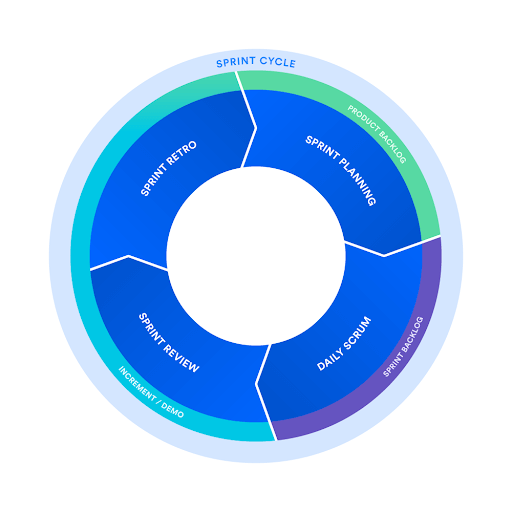
\includegraphics[height=12cm]{sprint-cycle}
      \caption{Ciclo di uno Sprint}
      \textbf{Fonte:} \href{https://www.atlassian.com}{atlassian.com}
    \end{center}
  \end{figure}
\vspace{20pt} 

\subsection{Strumeti a supporto dei processi}

\subsubsection{Git \& GitLab}
Git è un \emph{Distributed Version Control System}, \emph{open-source} e gratuito, progettato per gestire progetti di \
grandi e piccole dimensioni con efficienza. \\

GitLab, a differenza di git, è una piattaforma di \emph{hosting} per \emph{git repositories}; inoltre offre diversi servizi \
per la gestione del progetto, quali:

\begin{itemize}
  \item \emph{Issue Tracking System};
  \item \emph{Project Board}
  \item \emph{\acrfull{ci}};
  \item \emph{\acrfull{cd}}.
\end{itemize}

\vspace{20pt}
  \begin{figure}[!ht]
    \begin{center}
      
\includegraphics[height=3cm]{logo-gitlab}
      \caption{Logo GitLab}
      \textbf{Fonte:} \href{https://www.gitlab.com}{gitlab.com}
    \end{center}
  \end{figure}
\vspace{20pt} 

\subsubsection{\emph{Google Workspace}}
\emph{Google Workspace} è un insieme di strumenti di collaborazione e produttività sviluppato da Google. \
I servizi utilizzati maggiormente dall'azienda sono:

\begin{itemize}
  \item \emph{Gmail} per le comunicazioni formali;
  \item \emph{Calendar} per la gestione degli impegni aziendali;
  \item \emph{Drive} per la memorizzazione di file nel \emph{cloud};
  \item \emph{Meet} per le riunioni con i clienti;
  \item \emph{Google Docs Suite} per la creazione di documenti e presentazioni.
\end{itemize}

\vspace{20pt}
  \begin{figure}[!ht]
    \begin{center}
      
\includegraphics[width=10cm]{logo-google-workspace}
      \caption{Logo Google Workspace}
      \textbf{Fonte:} \href{https://workspace.google.com}{workspace.google.com}
    \end{center}
  \end{figure}
\vspace{20pt} 

%**************************************************************
\section{Rapporto con l'innovazione}
L'azienda è sempre aggiornata sulle nuove tecnologie partecipando ad incontri tecnologici con relatori di spicco: \emph{Google} e \emph{Amazon}, \
per citarne alcuni; e, in generale, è molto propensa all'innovazione accettando la presa in carico di progetti innovativi che sfruttano \
i moderni \emph{smart speakers}, l'architettura \emph{Serverless} o nell'ambito dell'\acrfull{iot}.             % L'azienda
% !TEX encoding = UTF-8
% !TEX TS-program = pdflatex
% !TEX root = ../tesi.tex

%**************************************************************
\chapter{Lo stage}
\label{cap:stage}
%**************************************************************
\section{Il progetto}
In questa sezione descrivo il progetto di stage e il perché mi è stato proposto. 

%**************************************************************
\section{Obiettivi}
In quest asezione descrivo gli obiettivi del progetto di stage.

%**************************************************************
\section{Vincoli}

\subsection{Vincoli di dominio}
In questa sezione descrivo i vincoli di dominio del progetto.

\subsection{Vincoli tecnologici}
In questa sezione descrivo i vincoli tecnologici del progetto.

\subsection{Vincoli metodologici}
In questa sezione descrivo i vincoli metodologici del progetto.

\subsection{Vincoli temporali}
In questa sezione descrivo i vincoli temporali del progetto.             % Lo stage
% !TEX encoding = UTF-8
% !TEX TS-program = pdflatex
% !TEX root = ../tesi.tex

%**************************************************************
\chapter{Sviluppo del progetto}
\label{cap:sviluppo}
%**************************************************************
\section{Analisi dei requisiti}
In questa sezione descrivo gli attori di sistema e come ho svolto l'analisi dei requisiti.
Quest'ultima, a sua volta, è suddivisa in due sotto-attività che sono: lo studio dei casi d'uso e la redazione delle \emph{user stories}.
Per ognuna di esse dedico una sezione e riporto solo le parti più rilevanti.

\subsection{Attori}
La figura \ref{fig:attori} riporta il diagramma \emph{\acrshort{uml}} che descrive la gerarchia degli attori del sistema. Dopo un'attenta analisi ho individuato: cinque \
attori principali e uno secondario. Gli attori principali da me individuati sono: l'utente non autenticato, l'utente non autorizzato, l'utente \
di tipo fornitore, l'utente di tipo personale e l'utente di tipo \emph{admin}. L'unico utente secondario che ho individuato è Google, in quanto, all'interno del sistema, \
utilizziamo \emph{Google SSO} come servizio di autenticazione. 

\begin{figure}[!ht]
  \begin{center}
    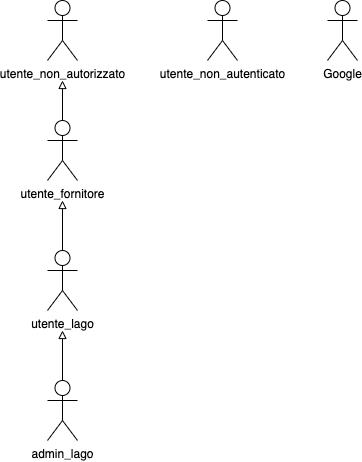
\includegraphics[scale=0.35]{usecase/attori}
    \caption{Gerarchia degli attori di sistema}
    \label{fig:attori}
  \end{center}
\end{figure}

\subsection{Casi d'uso}
Durante l'attività di analisi ho definito diversi diagrammi dei casi d'uso mediante il linguaggio \emph{\acrshort{uml}}. Tutti i diagrammi sono contenuti all'interno \
del documento Analisi dei Requisiti aziendale. In questa sezione mostrerò solo il caso d'uso più generale, per dare un'idea di ciò che è possibile fare all'interno \
dell'applicazione. Ogni caso d'uso segue la seguente denominazione:

\begin{center}
  UC[codice]
\end{center}

dove per [codice] si intende un identificativo univoco del caso d'uso riportato in forma gerarchica. Per ogni caso d'uso, inoltre, vengono specificati:
\begin{itemize}
  \item Gli attori coinvolti;
  \item Una breve descrizione;
  \item La precondizione;
  \item La postcondizione;
  \item Lo scenario principale;
  \item Le eventuali estensioni.
\end{itemize}

\subsubsection{Caso d'uso UC0 - Scenario principale}
\begin{figure}[!ht]
  \begin{center}
    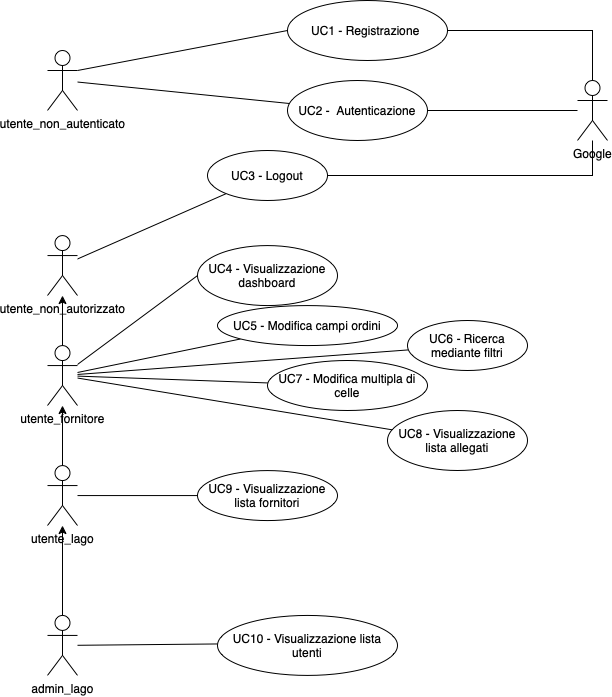
\includegraphics[scale=0.38]{usecase/main-scenario}
    \caption{UC0: Scenario principale}
    \label{fig:uc0}
  \end{center}
\end{figure}

\begin{itemize}
  \item \textbf{Attori:} utente non autenticato, utente autenticato, utente di tipo fornitore, utente di tipo personale e utente di tipo \emph{admin};
  \item \textbf{Descrizione:} nella schermata principale un utente non autenticato può autenticarsi, o registrarsi, tramite l'apposito pulsante che reindirizza l'utente al \emph{form} di Google. Un utente non autorizzato può effettuare il \emph{logout} dalla piattaforma. Un utente di tipo fornitore, oltre alle funzionalità dell'utente non autorizzato, ha la possibilità di:\
    \begin{itemize}
      \item visualizzare la \emph{dashboard};
      \item modificare una riga;
      \item effettuare la ricerca mediante filtri;
      \item effettuare la modifica multipla di cella;
      \item visualizzare gli allegati relativi ad un ordine.
    \end{itemize}
    Un utente di tipo personale, oltre alle funzionalità dell'utente fornitore, può visualizzare la lista dei fornitori. Un utente di tipo \emph{admin}, infine, oltre alle funzionalità dell'utente di tipo personale, può visualizzare la lista degli utenti registrati sulla piattaforma;
  \item \textbf{Precondizione:} il sistema è avviato e mostra la pagina principale dell'applicazione;
  \item \textbf{Postcondizione:} il sistema ha ricevuto tutte le informazioni dall'utente sulle operazioni che vuole eseguire;
  \item \textbf{Scenario principale:} 
    \begin{itemize}
      \item L'utente non autenticato può effettuare la registrazione alla piattaforma (UC1);
      \item L'utente non autenticato può effettuare l'autenticazione (UC2);
      \item L'utente non autorizzato, l'utente di tipo fornitore, l'utente di tipo personale e l'utente di tipo \emph{admin} possono effettuare il \emph{logout} (UC3);
      \item L'utente di tipo fornitore, l'utente di tipo personale e l'utente di tipo \emph{admin} possono visualizzare la \emph{dashboard} (UC4);
      \item L'utente di tipo fornitore, l'utente di tipo personale e l'utente di tipo \emph{admin} possono modificare un campo di un ordine (UC5);
      \item L'utente di tipo fornitore, l'utente di tipo personale e l'utente di tipo \emph{admin} possono effettuare la ricerca mediante filtri (UC6);
      \item L'utente di tipo fornitore, l'utente di tipo personale e l'utente di tipo \emph{admin} possono effettuare la modifica multipla di ordini (UC7);
      \item L'utente di tipo fornitore, l'utente di tipo personale e l'utente di tipo \emph{admin} possono visualizzare gli allegati di un ordine (UC8);
      \item L'utente di tipo personale e l'utente di tipo \emph{admin} possono visualizzare la lista dei fornitori (UC9);
      \item L'utente di tipo \emph{admin} può visualizzare la lista degli utenti registrati nella piattaforma (UC10).
    \end{itemize}
\end{itemize}

\subsection{\emph{User Stories}}
Grazie alla definizione dei casi d'uso ho estratto le \emph{user stories}, delle quali ho provveduto allo svolgimento delle attività in esse specificate durante il periodo di \emph{stage}. 
Di seguito sono riportate quelle relative alle funzionalità principali.

\subsubsection{Login con \emph{Google SSO} (5)}
Come utente non autenticato, voglio poter accedere alla piattaforma mediante \emph{Google SSO}. \\
\emph{Tasks:}
\begin{itemize}
  \item \emph{\Gls{backend}}:
    \begin{itemize}
      \item Creazione \emph{collection users};
      \item Implementazione chiamata \emph{\acrshort{api}} di \emph{Google SSO};
      \item Se l'utente non è presente, memorizzare il \emph{token} e metterlo in stato \emph{"disabled"};
      \item Verifica della validità del \emph{token}.
    \end{itemize}
  \item \emph{\Gls{frontend}}:
    \begin{itemize}
      \item Implementazione della chiamata all'\emph{\acrshort{api}} di \emph{login} del \emph{\gls{backend}};
      \item Creazione della sessione utente;
      \item Reindirizzamento alla \emph{dashboard}.
    \end{itemize}
\end{itemize}

\subsubsection{Visualizzazione lista fornitori (5)}
Come utente di tipo personale, voglio visualizzare la lista di tutti i fornitori abilitati. \\
\emph{Tasks:}
\begin{itemize}
  \item \emph{\Gls{backend}}:
    \begin{itemize}
      \item Creazione \emph{collection suppliers};
      \item Verifica dei permessi di esecuzione dell'\emph{\acrshort{api}};
      \item Implementazione dell'\emph{\acrshort{api} "get suppliers"}.
    \end{itemize}
  \item \emph{\Gls{frontend}}:
    \begin{itemize}
      \item Implementazione della chiamata all'\emph{\acrshort{api} "get suppliers"} del \emph{\gls{backend}};
      \item Visualizzazione della lista dei fornitori.
    \end{itemize}
\end{itemize}

\subsubsection{Visualizzazione fornitore (5)}
Come utente di tipo personale o utente di tipo fornitore, voglio visualizzare la griglia di un fornitore. \\
\emph{Tasks:}
\begin{itemize}
  \item \emph{\Gls{backend}}:
    \begin{itemize}
      \item Definizione della struttura della configurazione di una colonna;
      \item Definizione della struttura della configurazione per il contenuto della colonna;
      \item Creazione \emph{collection order-rows};
      \item Verifica dei permessi di esecuzione dell'\emph{\acrshort{api}};
      \item Implementazione dell'\emph{\acrshort{api} "get order-rows"} di un fornitore.
    \end{itemize}
  \item \emph{\Gls{frontend}}:
    \begin{itemize}
      \item Implementazione della chiamata all'\emph{\acrshort{api} "get order-rows"} del \emph{\gls{backend}};
      \item Visualizzazione della griglia con i dati degli ordini di un fornitore.
    \end{itemize}
\end{itemize}

\subsubsection{Modifica dei campi di un ordine (5)}
Come utente di tipo personale o utente di tipo fornitore, voglio poter modificare un campo di un ordine. \\
\emph{Tasks:}
\begin{itemize}
  \item \emph{\Gls{backend}}:
    \begin{itemize}
      \item Verifica dei permessi di esecuzione dell'\emph{\acrshort{api}};
      \item Implementazione dell'\emph{\acrshort{api} "update order-row"} per un ordine di un fornitore.
    \end{itemize}
  \item \emph{\Gls{frontend}}:
    \begin{itemize}
      \item Validazione del campo modificato;
      \item Visualizzazione di un errore in caso di valore non valido;
      \item Implementazione della chiamata all'\emph{\acrshort{api} "update order-row"} del \emph{\gls{backend}};
      \item Visualizzazione della griglia con i dati degli ordini aggiornati.
    \end{itemize}
\end{itemize}

\subsubsection{Visualizzazione della lista degli utenti (5)}
Come utente \emph{admin}, voglio poter visualizzare la lista degli utenti registrati. \\
\emph{Tasks:}
\begin{itemize}
  \item \emph{\Gls{backend}}:
    \begin{itemize}
      \item Verifica dei permessi di esecuzione dell'\emph{\acrshort{api}};
      \item Implementazione dell'\emph{\acrshort{api} "get users"}.
    \end{itemize}
  \item \emph{\Gls{frontend}}:
    \begin{itemize}
      \item Implementazione della chiamata all'\emph{\acrshort{api} "get users"} del \emph{\gls{backend}};
      \item Visualizzazione della lista degli utenti.
    \end{itemize}
\end{itemize}

\subsubsection{Visualizzazione della lista degli allegati (5)}
Come utente di tipo personale o utente di tipo fornitore, voglio poter visualizzare la lista degli allegati relativi ad un ordine. \\
\emph{Tasks:}
\begin{itemize}
  \item \emph{\Gls{backend}}:
    \begin{itemize}
      \item Verifica dei permessi di esecuzione dell'\emph{\acrshort{api}};
      \item Implementazione del sistema per l'invio dei file allegati da visualizzare;
      \item Implementazione dell'\emph{\acrshort{api} "get attachments"} di un ordine.
    \end{itemize}
  \item \emph{\Gls{frontend}}:
    \begin{itemize}
      \item Implementazione della chiamata all'\emph{\acrshort{api} "get attachments"} del \emph{\gls{backend}};
      \item Visualizzazione della lista degli allegati di un ordine.
    \end{itemize}
\end{itemize}

%**************************************************************
\section{Progettazione architetturale}

L'applicazione è costituita da due parti principali: il \emph{\gls{frontend}} e il \emph{\gls{backend}}, che costituiscono rispettivamente il \emph{client} e il \emph{server} nell'architettura \emph{client-server}. \
All'interno di questa architettura, il \emph{\gls{frontend}} ha il compito di interagire con l'utente e di mostrare i dati ottenuti dal \emph{server}. Il \emph{\gls{backend}}, invece, fornisce le \emph{\acrshort{api}} \
per poter svolgere determinate operazioni e ottenerne i risultati. Come si può vedere dalla figura \ref{fig:client-server}, che raffigura il flusso di comunicazione in questa architettura, entrambi i componenti sono indipendenti tra loro e comunicano utilizzando richieste \emph{\acrshort{http}}. Possono essere di diversi tipi a \
seconda dell'operazione che intendiamo svolgere: 
\begin{itemize}
  \item \textbf{\emph{GET}:} per ottenere i dati dal \emph{server};
  \item \textbf{\emph{POST}:} per caricare dei dati sul \emph{server};
  \item \textbf{\emph{PUT}:} per aggiornare i dati sul \emph{server};
  \item \textbf{\emph{DELETE}:} per eliminare dei dati sul \emph{server}.
\end{itemize} 

\begin{figure}[!ht]
  \begin{center}
    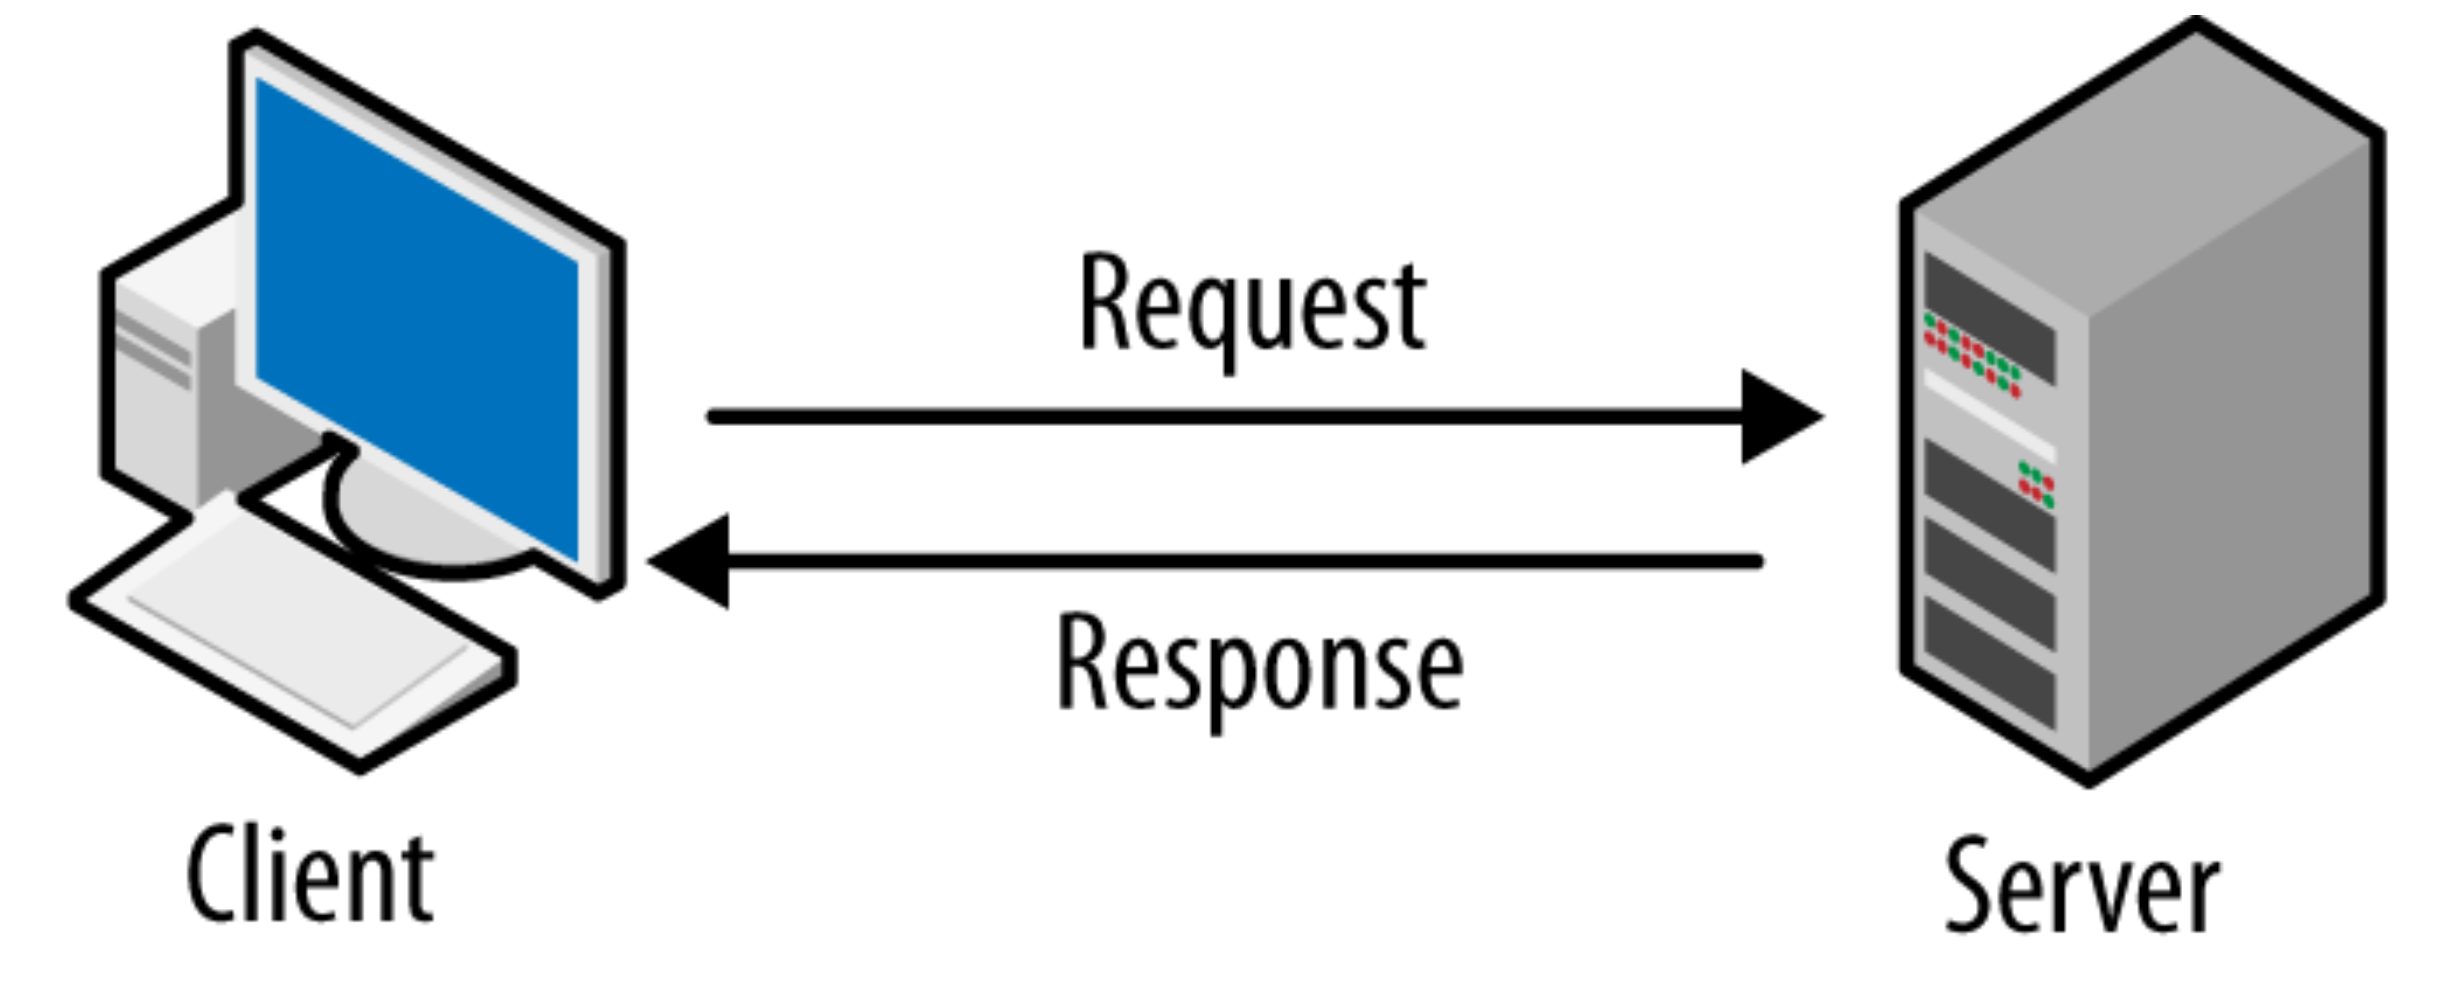
\includegraphics[scale=0.1]{design/client-server}
    \caption{Flusso di comunicazione \emph{client-server}}
    \label{fig:client-server}
  \end{center}
\end{figure}

Come si evince dalla figura \ref{fig:general-design}, che mostra lo schema architetturale generale, l'applicazione è costituita da tre \emph{packages} principali:
\begin{itemize}
  \item \textbf{\emph{edi-api}:} contiene i \emph{packages} necessari, per il funzionamento del \emph{\gls{backend}};
  \item \textbf{\emph{edi-ui}:} contiene i \emph{packages} necessari, per il funzionamento del \emph{\gls{frontend}};
  \item \textbf{\emph{edi-commons}:} contiene i \emph{packages}, che vengono riutilizzati sia nel \emph{\gls{backend}} che nel \emph{\gls{frontend}}.
\end{itemize}

\begin{figure}[!ht]
  \begin{center}
    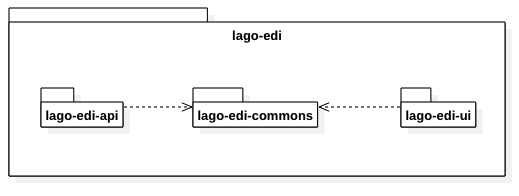
\includegraphics[scale=1, width=\textwidth]{design/general}
    \caption{Architettura generale dell'applicazione}
    \label{fig:general-design}
  \end{center}
\end{figure}
\newpage

L'applicazione, per funzionare, necessita dell'utilizzo di alcune librerie e \emph{frameworks} esterni. Questi garantiscono l'utilizzo di alcune funzionalità che \
permettono di velocizzare il lavoro e di svolgerlo in maniera più ordinata e sicura. Quelli che ho utilizzato all'interno del progetto, suddivisi per \emph{package}, sono:
\begin{itemize}
  \item \textbf{edi-api}
    \begin{itemize}
      \item \textbf{\emph{express}:} è il \emph{framework} su cui si basa l'intera applicazione \emph{\gls{backend}}, fornisce le basi per la creazione del \emph{server} e del \emph{routing};
      \item \textbf{\emph{mongoose}:} è una libreria per creare i modelli degli oggetti che vengono memorizzati su \emph{\textbf{MongoDB}}, inoltre, permette di eseguire le \emph{query} per manipolare i dati del \emph{database};
      \item \textbf{\emph{passport}:} è una libreria che rende disponibile dei \emph{middlewares} per facilitare l'implementazione dell'autenticazione su applicazioni basate su \emph{\textbf{express}};
      \item \textbf{\emph{inversify}:} è una libreria che permette di implementare applicazioni che sfruttano il \emph{design pattern Dependency Injection} con \emph{\acrfull{ioc}};
      \item \textbf{\emph{googleapis}:} è una libreria utilizzata per usufruire delle \emph{\acrshort{api}} di Google. Nello specifico, ho utilizzato questa libreria per implementare l'autenticazione degli utenti;
      \item \textbf{\emph{joi}:} è una libreria che permette di definire degli schemi per validare i dati in ingresso.
    \end{itemize}
  \item \textbf{edi-ui}
    \begin{itemize}
      \item \textbf{\emph{fuse.js}:} è una libreria che facilita l'implementazione delle funzionalità di ricerca lato \emph{\gls{frontend}};
      \item \textbf{\emph{styled-components}:} è una libreria che consente di definire dei componenti per la \emph{\gls{ui}} riutilizzabili e con stile personalizzato, senza l'utilizzo di file dedicati riducendo le dimensioni del progetto;
      \item \textbf{\emph{react-data-grid}:} è una libreria che fornisce i componenti per la creazione di griglie, uno dei componenti più importanti dell'applicazione \emph{\gls{frontend}};
      \item \textbf{\emph{react-query}:} è una libreria per applicazioni basate su \emph{\textbf{React}}, che fornisce le primitive di rete, per poter interagire con il \emph{\gls{backend}};
      \item \textbf{\emph{formik}:} è una libreria per applicazioni basate su \emph{\textbf{React}}, che facilita la creazione di \emph{form} per l'invio di dati inseriti dall'utente;
      \item \textbf{\emph{react}:} è la libreria su cui si basa l'intera applicazione \emph{\gls{frontend}}, permette la realizzazione di \emph{\acrfullpl{ui}} basate su componenti.
    \end{itemize}
\end{itemize} 

%**************************************************************
\section{Progettazione di dettaglio}

\subsection{Architettura del \emph{\gls{backend}}}
Addentrandoci nell'architettura del \emph{package} \textbf{edi-api}, come mostra la figura \ref{fig:be-design}, possiamo notare come esso sia costituito dai seguenti \emph{packages}:
\begin{itemize}
  \item \textbf{\emph{controllers}:} contiene tutti i componenti per fornire una risposta alle richieste \emph{\acrshort{http}} in ingresso. Costituisce la \emph{application logic};
  \item \textbf{\emph{middlewares}:} contiene tutte le funzioni da eseguire prima dell'esecuzione del \emph{controller};
  \item \textbf{\emph{services}:} contiene tutti i componenti necessari per fornire un servizio ai \emph{controllers};
  \item \textbf{\emph{repositories}:} contiene tutti i componenti che si occupano di interagire con il \emph{database};
  \item \textbf{\emph{models}:} contiene tutte le classi che costituiscono le tipologie di dati utilizzati nell'applicazione.
\end{itemize}

\begin{figure}[!ht]
  \begin{center}
    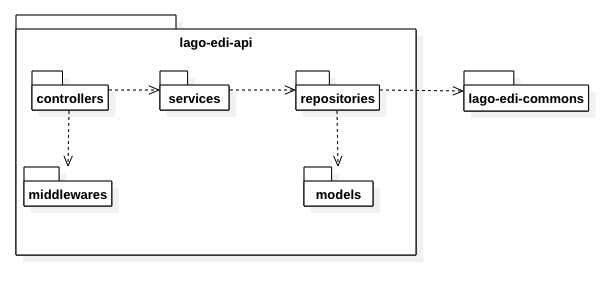
\includegraphics[scale=0.45]{design/backend}
    \caption{Architettura del \emph{\gls{backend}}}
    \label{fig:be-design}
  \end{center}
\end{figure}

\subsubsection{\emph{Design pattern} utilizzati}
Di seguito descrivo i \emph{design pattern} che ho utilizzato nell'architettura del \emph{\gls{backend}}. 
Per ognuno di essi descrivo lo scopo dell'utilizzo e il contesto di applicazione fornendo, inoltre, un diagramma che ne dimostri l'applicazione.
\begin{itemize}
  \item \textbf{\emph{\acrlong{mvc}}:} 
  la figura \ref{fig:mvc-pattern} fornisce una rappresentazione grafica del \emph{design pattern} architetturale \emph{\acrshort{mvc}}. Quest'ultimo, viene utilizzato per mantenere separati i compiti dei diversi componenti,
  che interpretano i tre ruoli principali: \emph{Model, View} e \emph{Controller}. Nel contesto applicativo, il \emph{pattern \acrshort{mvc}}, costituisce l'architettura generale del \emph{\gls{backend}}, questo perché il
  \emph{framework \textbf{express}} è basato su tale architettura. Durante l'implementazione non è stata implementata alcuna \emph{view}, in quanto, il \emph{\gls{backend}} si preoccupa esclusivamente di rendere disponibili 
  le \emph{\acrshort{api}} al \emph{\gls{frontend}} e quindi, risulta inutile, per questo motivo nella figura sottostante è evidenziata in rosso.

  \begin{figure}[!ht]
    \begin{center}
      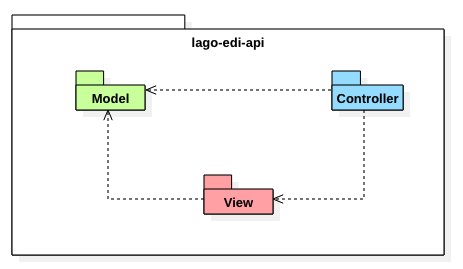
\includegraphics[scale=0.45]{design/patterns/mvc}
      \caption{Contesto di utilizzo del \emph{design pattern \acrshort{mvc}}}
      \label{fig:mvc-pattern}
    \end{center}
  \end{figure}
  \item \textbf{\emph{Dependency Injection}:}
  la figura \ref{fig:di-pattern} rappresenta il diagramma delle classi del \emph{design pattern} architetturale \emph{Dependency Injection}. Questo \emph{design pattern} è utilizzato per separare il comportamento di un componente dalla 
  risoluzione delle sue dipendenze, le quali, in questo modo, vengono minimizzate. Nel contesto applicativo, viene impiegato nell'architettura generale del
  \emph{package} \textbf{edi-api} per ottenere \emph{software} più facile da testare e manutenere. 

  \begin{figure}[!ht]
    \begin{center}
      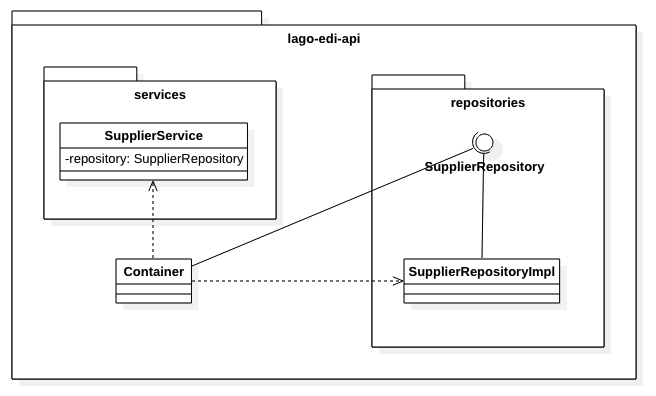
\includegraphics[scale=0.30]{design/patterns/di}
      \caption{Contesto di utilizzo del \emph{design pattern Dependency Injection}}
      \label{fig:di-pattern}
    \end{center}
  \end{figure}
\end{itemize}

\newpage
\subsection{Architettura del \emph{\gls{frontend}}}
La figura \ref{fig:fe-design} fornisce una rappresentazione grafica dell'architettura relativa al \emph{\gls{frontend}}. \
Il \emph{package} \textbf{edi-ui} è composto dai seguenti \emph{subpackages}:
\begin{itemize}
  \item \textbf{\emph{views}:} contiene tutte le pagine che il \emph{\gls{frontend}} deve mostrare all'utente;
  \item \textbf{\emph{contexts}:} contiene tutte le classi per gestire lo stato globale;
  \item \textbf{\emph{services}:} contiene tutti i componenti necessari per ottenere i dati dal \emph{\gls{backend}};
  \item \textbf{\emph{components}:} contiene tutti i componenti necessari per il \emph{rendering} delle pagine;
  \item \textbf{\emph{interfaces}:} contiene tutte le interfacce per la configurazione dei componenti della \emph{view}.
\end{itemize}

\begin{figure}[!ht]
  \begin{center}
    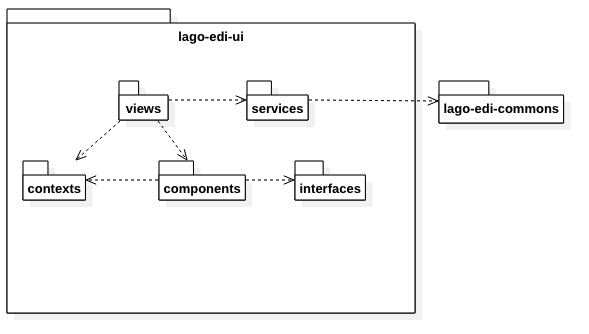
\includegraphics[scale=0.45]{design/frontend}
    \caption{Architettura del \emph{\gls{frontend}}}
    \label{fig:fe-design}
  \end{center}
\end{figure}

\subsubsection{\emph{Design pattern} utilizzati}
Di seguito descrivo i \emph{design pattern} che ho utilizzato nell'architettura del \emph{\gls{frontend}}. 
Per ognuno di essi descrivo lo scopo dell'utilizzo e il contesto di applicazione fornendo, inoltre, un diagramma che ne dimostri l'applicazione.
\begin{itemize}
  \item \textbf{\emph{Builder}:}
  la figura \ref{fig:builder-pattern} mostra il diagramma relativo al \emph{design pattern} creazionale \emph{Builder}. Questo \emph{design pattern}, permette di separare la costruzione di un oggetto complesso dalla
  sua rappresentazione e fornisce un controllo migliore del processo di costruzione, in quanto fornisce una costruzione \emph{step-by-step}. Nel contesto applicativo, è impiegato per la creazione delle colonne
  che compongono la griglia di un fornitore. Grazie al suo utilizzo, l'applicazione sarà in grado di creare nuove tipologie di colonne, senza apportare eccessive modifiche.

  \begin{figure}[!ht]
    \begin{center}
      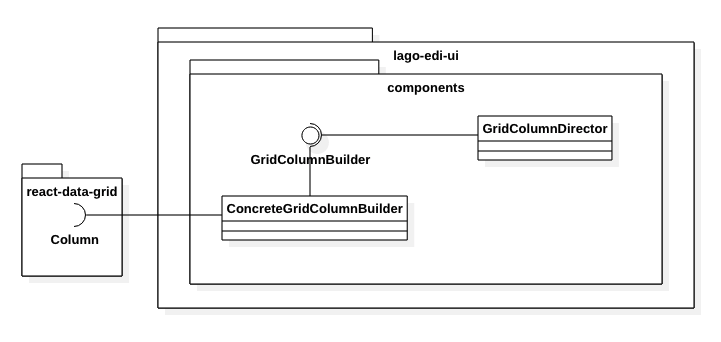
\includegraphics[scale=0.35]{design/patterns/builder}
      \caption{Contesto di utilizzo del \emph{design pattern Builder}}
      \label{fig:builder-pattern}
    \end{center}
  \end{figure}
  \newpage
  \item \textbf{\emph{Factory}:}
  la figura \ref{fig:factory-pattern} mostra il diagramma relativo al \emph{design pattern} creazionale \emph{Factory}. Quest'ultimo separa la creazione di un oggetto dalla sua rappresentazione, senza esporre la logica 
  di creazione. Nel contesto applicativo, viene adottato per la costruzione dei seguenti componenti della griglia del fornitore: 
  \begin{itemize}
    \item le celle;
    \item gli \emph{editor} delle celle;
    \item i \emph{formatter} delle celle.
  \end{itemize}

  \begin{figure}[!ht]
    \begin{center}
      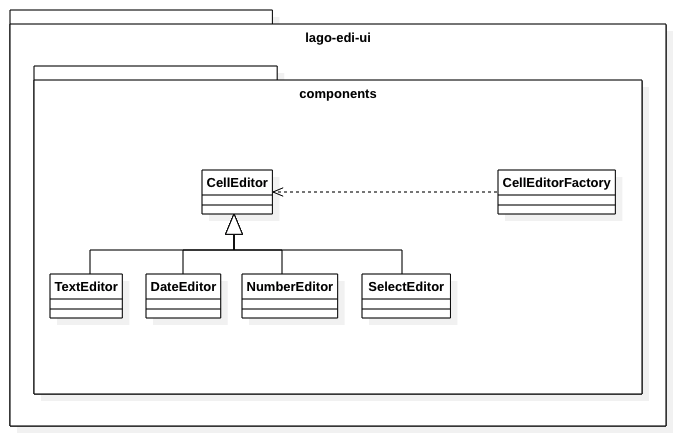
\includegraphics[scale=0.35]{design/patterns/factory}
      \caption{Contesto di utilizzo del \emph{design pattern Factory}}
      \label{fig:factory-pattern}
    \end{center}
  \end{figure}
\end{itemize}

\subsection{Struttura del \emph{database}}
Come \emph{database} ho utilizzato il \emph{\acrshort{dbms} NoSQL \textbf{MongoDB}}, mentre, per interagire con esso, ho impiegato la libreria \textbf{mongoose}. 
La figura \ref{fig:db-design} mostra il diagramma \emph{\acrshort{er}} del \emph{database} che ho realizzato utilizzando l'applicazione \textbf{\href{https://dbdiagram.io/}{dbdiagram.io}}. 
Di seguito fornisco una breve descrizione di ogni \emph{collection} del \emph{database}:

\begin{itemize}
  \item \textbf{\emph{users}:} memorizza tutti i dati degli utenti, compreso il fornitore a cui ha accesso, nel caso esso sia di tipo fornitore;
  \item \textbf{\emph{suppliers}:} memorizza i dati dei fornitori, inclusa la configurazione delle colonne della tabella;
  \item \textbf{\emph{order\_rows}:} memorizza i dati di tutti gli ordini relativi ad ogni fornitore.
\end{itemize}

\begin{figure}[!ht]
  \begin{center}
    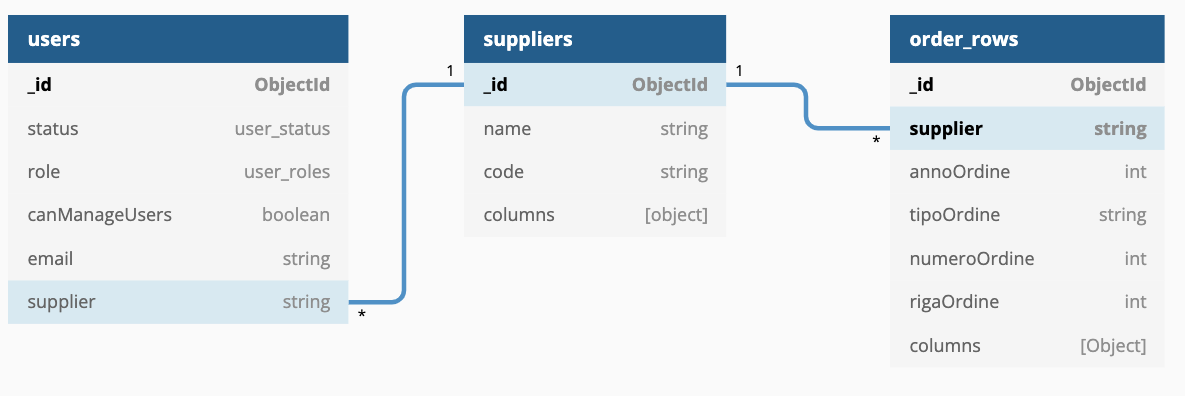
\includegraphics[scale=0.28]{design/database}
    \caption{Schema del \emph{database}}
    \label{fig:db-design}
  \end{center}
\end{figure}

\subsection{Diagrammi di sequenza}
Questa sezione riporta uno dei diagrammi di sequenza realizzati, durante il periodo di \emph{stage}, mediante l'utilizzo del \emph{software \textbf{StarUML}}.
La figura \ref{fig:auth-sequence} mostra il diagramma di sequenza relativo all'autenticazione, il più importante che ho realizzato, e che mi ha permesso di implementare la soluzione migliore possibile.

\begin{figure}[!ht]
  \begin{center}
    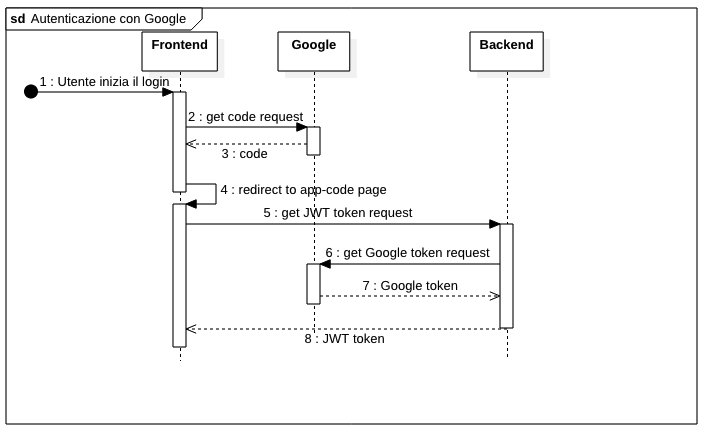
\includegraphics[scale=1, width=\textwidth]{design/auth-sequence}
    \caption{Diagramma di sequenza per l'autenticazione con Google}
    \label{fig:auth-sequence}
  \end{center}
\end{figure}

%**************************************************************
\section{Verifica e validazione}
In questa sezione descrivo le attività di verifica e validazione, svolte durante il periodo di \emph{stage}.
L'attività di verifica, a sua volta, è suddivisa in due sotto-attività che sono: l'analisi statica e l'analisi dinamica, per ognuna delle quali dedico una sezione.

\subsection{Analisi statica}
L'analisi statica permette di valutare la correttezza dei componenti, senza la loro esecuzione.
Durante il processo di sviluppo, ho utilizzato alcuni strumenti di analisi statica, per individuare gli errori più facilmente. Di seguito fornisco un elenco degli strumenti utilizzati:
\begin{itemize}
  \item \textbf{\textbf{WebStorm}:} questo \emph{\acrshort{ide}} permette di visualizzare \emph{warning} ed errori presenti all'interno del codice;
  \item \textbf{\textbf{ESLint}:} è un \emph{tool} che permette di trovare degli errori nel codice, basandosi su regole definite in fase di configurazione.
\end{itemize}
Grazie all'utilizzo di questi strumenti, sono riuscito a risolvere diversi problemi che ho avuto durante lo sviluppo del \emph{\gls{frontend}} e nell'utilizzo della libreria \emph{\textbf{Mongoose}}.
\textbf{\emph{WebStorm}}, inoltre, fornisce la funzionalità di analizzare il testo scritto, permettendo l'implementazione di pagine web senza errori di scrittura.

\subsection{Analisi dinamica}
L'analisi dinamica consente di valutare la correttezza dei componenti durante la sua esecuzione. 
È uno degli aspetti principali del processo di verifica. 
Questa attività viene svolta, principalmente, mediante l'esecuzione di \emph{tests} che possono essere di diversi tipi: di unità, di integrazione e di sistema.
Durante il periodo di \emph{stage} ho implementato solo \emph{test} di unità, a causa del poco tempo a disposizione per completare il lavoro.
Questo tipo di \emph{test}, ha lo scopo di verificare il corretto funzionamento della più piccola unità di \emph{software}.
Per la loro implementazione ho utilizzato il \emph{framework \textbf{Jest}}. Ogni test è strutturato nel seguente modo:

\begin{enumerate}
  \item Si definisce il gruppo dei \emph{tests} da implementare mediante la funzione \textbf{\emph{describe}}:
  \item Vengono invocate le funzioni \textbf{\emph{beforeAll}, \emph{beforeEach}, \emph{afterAll}, \emph{afterEach}}. per configurare le variabili necessarie e fare il \emph{mocking} delle dipendenze;
  \item Si definiscono i \emph{test} da eseguire mediante l'invocazione della funzione \emph{\textbf{it}};
  \item All'interno del \emph{test}, si invoca la funzione \emph{\textbf{describe}}, per definire l'esito atteso.
\end{enumerate}

La porzione di codice \ref{code:test-structure} mostra come ho strutturato i \emph{tests} durante lo \emph{stage}.

\begin{lstlisting}[caption=Esempio di struttura di \emph{test}, label={code:test-structure}, captionpos=b]
  describe("Testing UploadUsersValidator", () => {

    beforeAll(async () => {
      // moking delle dipendenze e configurazione delle variabili
      return 
    })

    // Eventuale invocazione di:
    //  - beforeEach
    //  - afterEach
    //  - afterAll

    it("Call with wrong role value should throw error", async () => {
      // implementazione test
    })
  })
\end{lstlisting}

%**************************************************************
\section{Prodotto finale}
L'applicazione implementata durante il periodo di \emph{stage} fornisce all'azienda committente, e ai suoi fornitori, una \emph{dashboard} per la visualizzazione degli ordini in ingresso e in uscita.
Ci sono diverse tipologie di utenti, ognuna delle quali può eseguire le proprie funzionalità specifiche previa autenticazione. 

\subsection{\emph{Login}}
Per poter accedere all'applicazione è necessario prima effettuare l'accesso, implementato mediante \emph{\textbf{Google SSO}}. 
È perciò necessario, che tutti gli utenti siano in possesso di un account Google.
Se l'utente svolge quest'operazione per la prima volta, verranno inseriti i suoi dati nel \emph{database} e dovrà attendere, che un \emph{admin} lo abiliti.
Solo dopo l'abilitazione potrà accedere all'applicazione e visualizzare la propria \emph{dashboard}. 
Nel caso, l'utente, non sia ancora abilitato viene visualizzato un errore.

\subsection{Fornitori}
L'utente di tipo fornitore è l'utente che può svolgere solo le funzionalità di base.
La figura \ref{fig:dashboard} mostra l'unica pagina che, l'utente, può visualizzare, ovvero, la \emph{dashboard}.
Quest'ultima rappresenta l'\emph{homepage} per questa tipologia di utente, per le altre tipologie sarà differente.
In questa pagina troviamo il componente principale dell'applicazione: la griglia con i dati degli ordini.
Con questo componente l'utente può svolgere le seguenti operazioni:

\begin{itemize}
  \item \textbf{Modifica di un valore:} le celle che permettono la modifica di un valore, sono evidenziate da un bordo verde. Per iniziare la modifica, e quindi mostrare il relativo \emph{editor}, ci sono due modalità: mediante il doppio \emph{click} con il \emph{mouse} o mediante l'immissione di caratteri da tastiera. Se al termine della modifica, alla pressione del pulsante "Invio", il valore non rispetta i limiti definiti durante la configurazione, l'intera riga sarà evidenziata in rosso.
  \item \textbf{Ricerca mediante filtri:} i campi di \emph{input} per poter filtrare le colonne, sono situati nell'\emph{header} della tabella, in corrispondenza della colonna a cui fanno riferimento. Questi campi di \emph{default} sono nascosti, e si possono rendere visibili mediante l'apposito pulsante in alto a destra: "Filtri". Si possono applicare più filtri contemporaneamente e il risultato sarà l'intersezione di ogni risultato;
  \item \textbf{Modifica multipla di una colonna:} è possibile, mediante \emph{drag-and-drop} verticale, copiare il valore della cella selezionata inizialmente in tutte le celle fino a quella in cui terminiamo la \emph{gesture};
  \item \textbf{Visualizzazione degli allegati:} nella colonna "Allegati" è presente un pulsante che permette di accedere alla finestra di gestione degli allegati. Fornisce, inoltre, il numero di allegati presenti per quel determinato ordine. La figura \ref{fig:attachments-list} mostra la lista degli allegati. Premendo il pulsante "Visualizza", relativo ad un allegato, possiamo scaricare il file per visionarlo;
  \item \textbf{Caricamento di un file allegato:} passando alla sezione "Carica allegato", dalla finestra degli allegati in figura \ref{fig:attachments-list}, è possibile effettuare il caricamento del file mediante l'apposito \emph{form}.
\end{itemize}

\begin{figure}[!ht]
  \begin{center}
    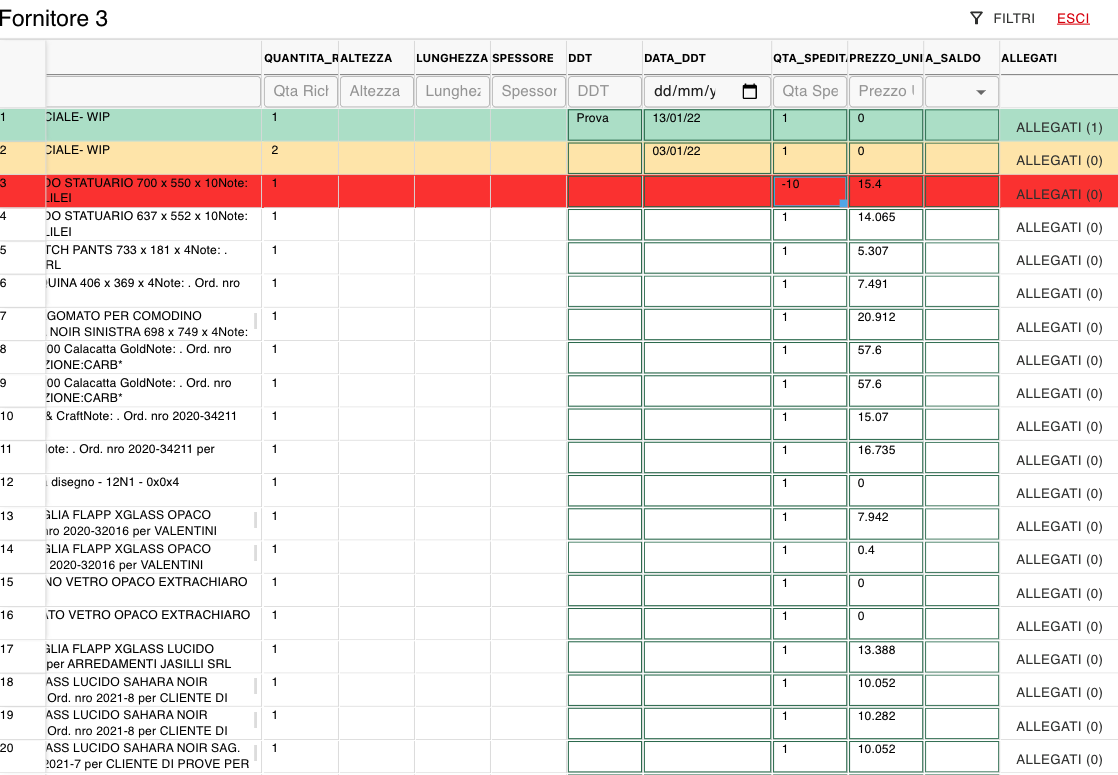
\includegraphics[scale=0.32, width=\textwidth]{screenshots/edi-user-dashboard.png}
    \caption{\emph{Dashboard} per l'utente di tipo fornitore}
    \label{fig:dashboard}
  \end{center}
\end{figure}

\newpage
\begin{figure}[!ht]
  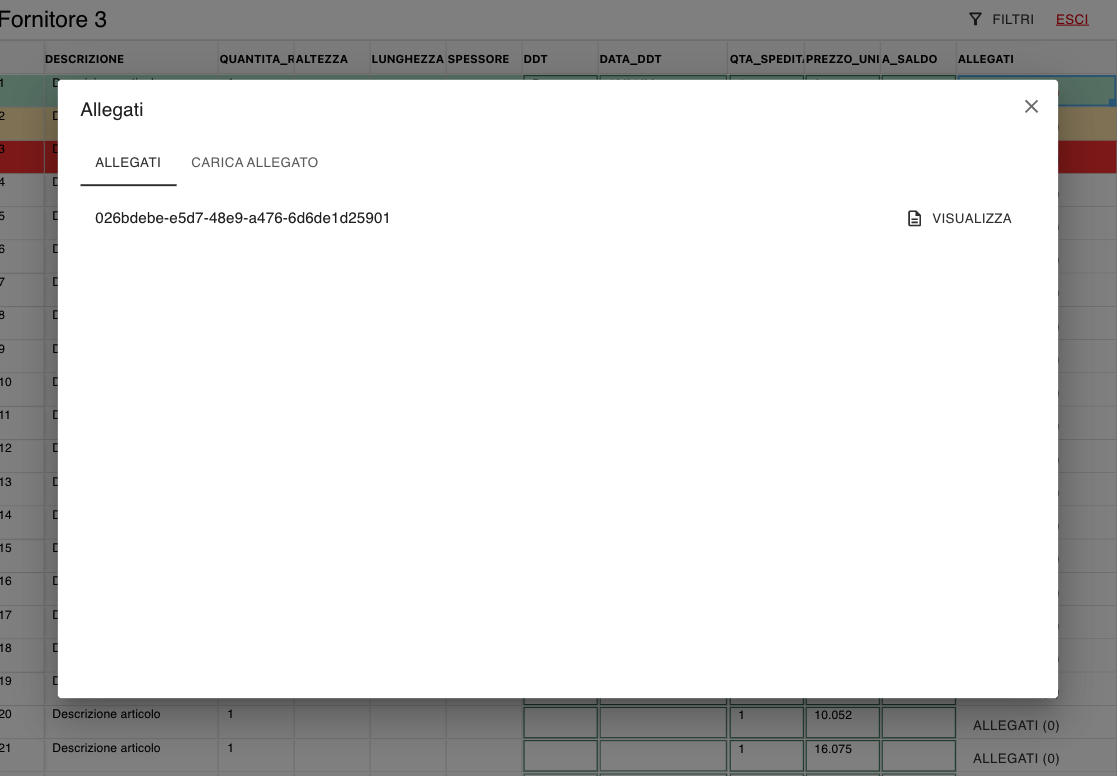
\includegraphics[scale=0.32]{screenshots/attachments-list.png}
  \caption{Lista degli allegati per un ordine}
  \label{fig:attachments-list}
  \centering
\end{figure}

\subsection{Personale}
Un utente facente parte del personale aziendale, la prima pagina che visualizza, come per gli utenti di tipo fornitore, è la \emph{dashboard}.
A differenza loro, però, come si osserva dalla figura \ref{fig:lago-dashboard}, mostra la lista di tutti i fornitori.
Per ogni fornitore nella lista è possibile visionare la relativa griglia degli ordini.
È possibile, inoltre, ricercare i fornitori mediante l'apposito campo di \emph{input}, situato sopra la lista.

\newpage
\begin{figure}[!ht]
  \begin{center}
    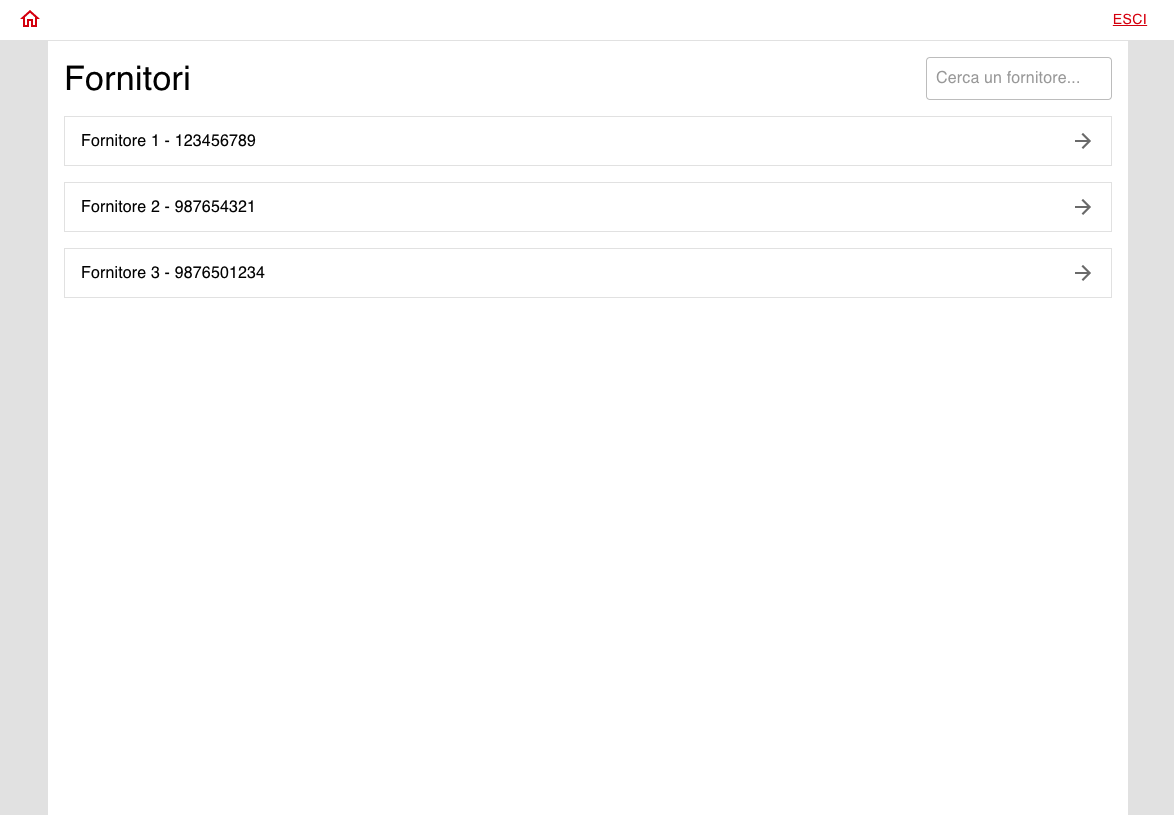
\includegraphics[scale=0.25, width=\textwidth]{screenshots/suppliers-list.png}
    \caption{\emph{Dashboard} per gli utenti di tipo personale}
    \label{fig:lago-dashboard}
  \end{center}
\end{figure}

Un'altra funzionalità di cui godono gli utenti di tipo personale, è la possibilità di passare alla visualizzazione degli ordini di un altro fornitore direttamente dalla griglia.
La figura \ref{fig:supplier-swicher} mostra il componente che rende possibile questa operazione.

\begin{figure}[!ht]
  \begin{center}
    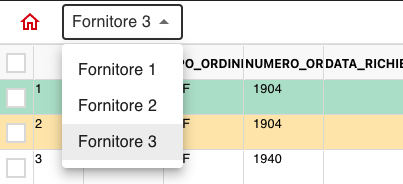
\includegraphics[scale=0.45]{screenshots/supplier-swicher.png}
    \caption{Componente per il cambio di fornitore dalla griglia}
    \label{fig:supplier-swicher}
  \end{center}
\end{figure}

La funzionalità, che risulta essere più importante però, è la possibilità di eliminare uno, o più, ordini dalla griglia.
Per potere fare ciò, è necessario prima selezionare tutti gli ordini che si intende eliminare, successivamente, si preme l'apposito pulsante, situato nella parte alta dell'applicazione, il quale apre una finestra di dialogo che richiede una conferma da parte dell'utente.
Una volta confermato, gli ordini selezionati verranno eliminati, mentre, in caso di annullamento, non sarà apportata alcuna modifica.
La figura \ref{fig:lago-grid-delete}, mostra gli ordini selezionati, pronti per poter essere eliminati.

\begin{figure}[!ht]
  \begin{center}
    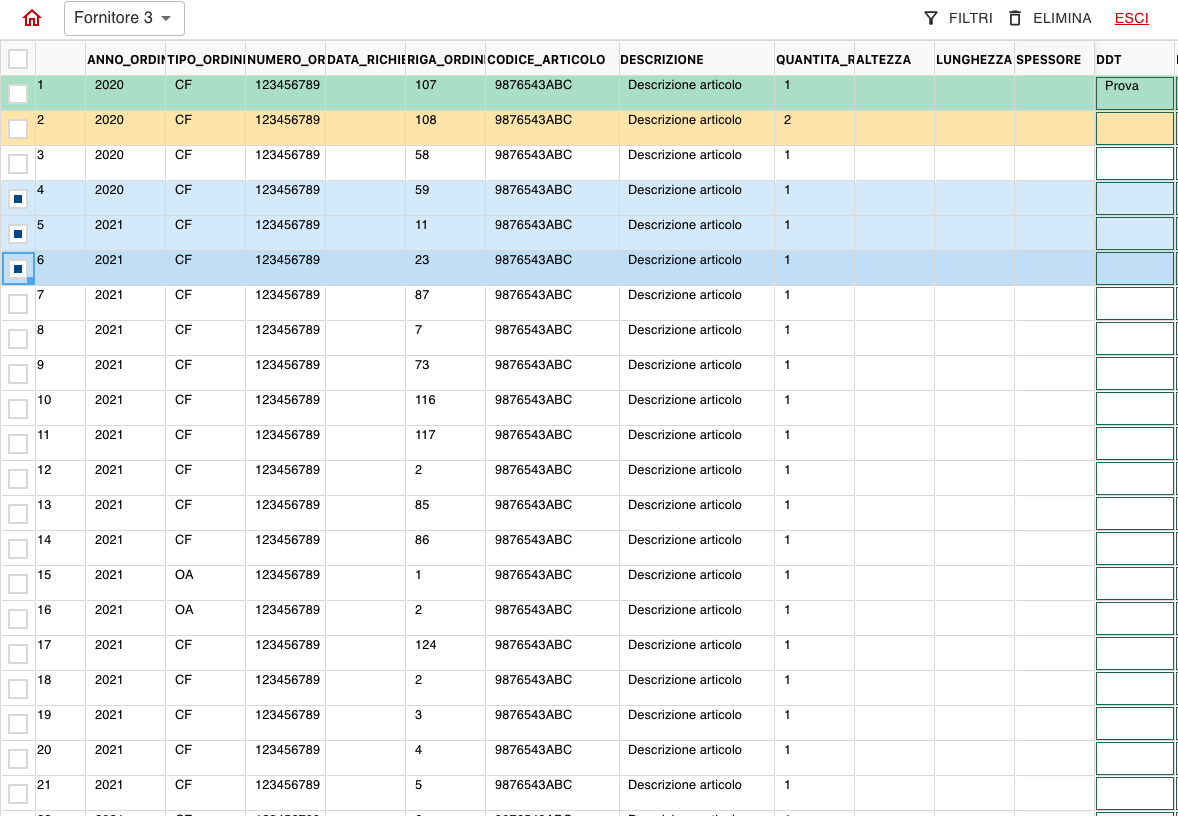
\includegraphics[scale=0.45, width=\textwidth]{screenshots/lago-grid-delete.png}
    \caption{Griglia con gli ordini da eliminare}
    \label{fig:lago-grid-delete}
  \end{center}
\end{figure}

\subsection{Amministratori}
Gli utenti amministratori si differenziano degli altri in quanto hanno la possibilità di gestire gli utenti.
La \emph{dashboard} relativa a questo tipo di utenza, ha una struttura molto minimale, è costituita da due \emph{tabs} per accedere o alla lista degli utenti o alla lista dei fornitori.
La funzionalità più importante, è la possibilità di abilitare un utente. 
Ciò è possibile mediante l'apposito \emph{form}, presente all'interno della figura \ref{fig:users-list}, che diventa modificabile dopo che viene premuto il pulsante "Modifica".
Questo \emph{form} consente, inoltre, la possibilità di cambiare il ruolo dell'utente e, se l'utente è di tipo personale, renderlo un \emph{admin}, oppure, se è di tipo fornitore, assegnargli la visualizzazione dei propri ordini.

\begin{figure}[!ht]
  \begin{center}
    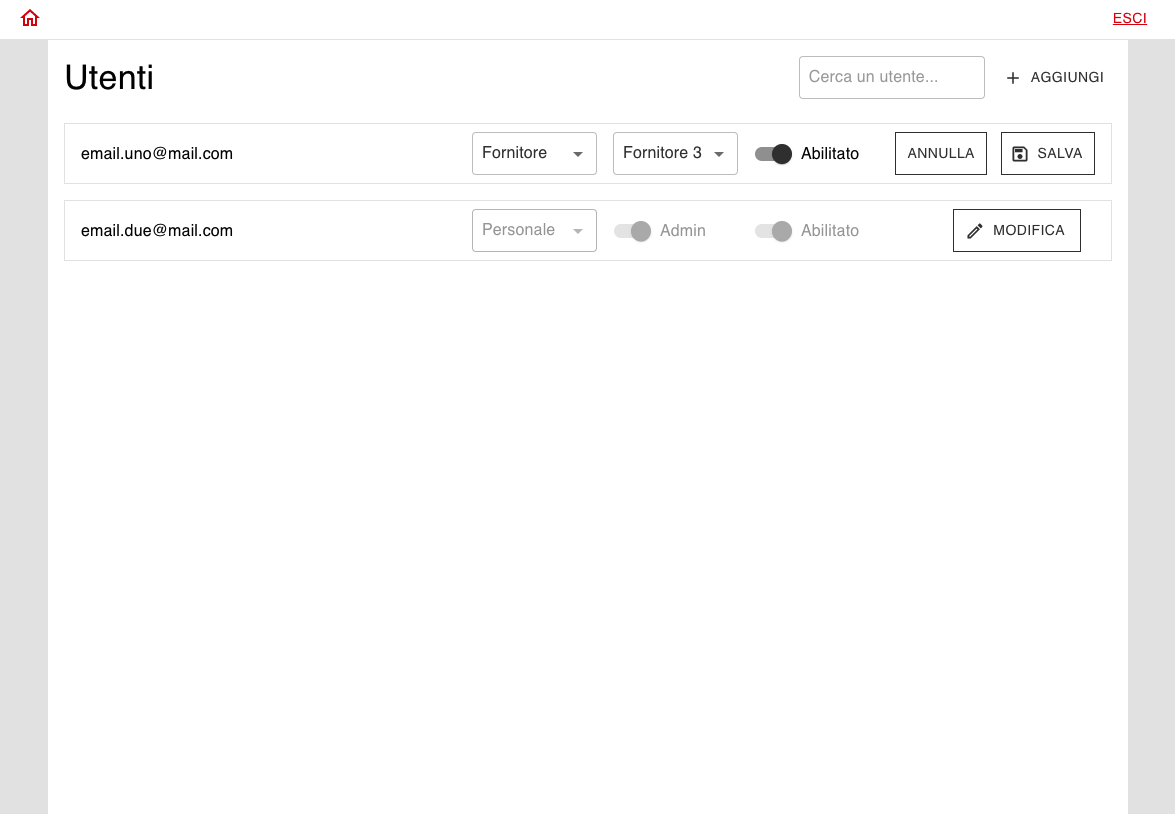
\includegraphics[scale=0.45, width=\textwidth]{screenshots/users-list.png}
    \caption{Lista degli utenti}
    \label{fig:users-list}
  \end{center}
\end{figure}

Un'altra funzionalità possibile per gli amministratori, è l'inserimento di uno, o più, nuovi utenti.
Ciò è possibile mediante l'apposito \emph{form}, visibile dopo aver premuto sul pulsante "Aggiungi".             % Implementazione del progetto
% !TEX encoding = UTF-8
% !TEX TS-program = pdflatex
% !TEX root = ../tesi.tex

%**************************************************************
\chapter{Valutazione retrospettiva}
\label{cap:valutazione}
%**************************************************************
\section{Resoconto degli obbiettivi aziendali raggiunti}

\subsection{Funzionalità dell'applicazione}
Al termine del periodo di \emph{stage} posso affermare di avere soddisfatto tutti gli obiettivi definiti dall'azienda prima di inziare il progetto.
Ho implementato tutte le funzionalità ritenute obbligatorie per la prima \emph{release} dell'applicazione, ovvero:
\begin{itemize}
  \item l'autenticazione degli utenti mediante \emph{\textbf{Google SSO}};
  \item la ricerca degli ordini mediante filtri;
  \item la modifica singola di un campo di un ordine;
  \item la modifica multipla mediante \emph{drag-and-drop} di un campo di più ordini;
  \item il blocco di colonne e impedirne lo \emph{scroll} orizzontale;
  \item l'eliminazione di uno o più ordini, se l'utente è in possesso dei permessi necessari.
\end{itemize}

Ho implementato, inoltre, le funzionalità ritenute facoltative, ovvero:
\begin{itemize}
  \item la gestione degli utenti;
  \item il caricamento e visualizzazione dei file allegati agli ordini.
\end{itemize}

Ciò è stato possibile grazie allo svolgimento di tutte le attività specificate nelle 16 \emph{user stories}, 12 delle quali obbligatorie e 8 facoltative. 

\subsection{Formazione}
Grazie a questa esperienza di \emph{stage} ho avuto la possibilità di imparare nozioni nuove e di approfondirne altre.
Il mio bagaglio tecnologico si è arricchito delle seguenti tecnologie:
\begin{itemize}
  \item \textbf{\emph{NodeJS}:} questa tecnologia l'avevo già usata in passato ma, grazie allo \emph{stage}, ho potuto apprendere quali sono le \emph{best practices} e approfondire le conoscenze a riguardo. Ho notato, inoltre, una diversa metodologia di approccio rispetto a quella usata durante le mie prime esperienze;
  \item \textbf{\emph{MongoDB}:} di questa tecnologia, prima dello \emph{stage}, ne avevo solamente sentito parlare e mi ha sempre incuriosito. Durante questo periodo ho avuto la possibilità di avvicinarmi al mondo dei \emph{database} non relazionali, imparando il loro funzionamento e le regole per una buona progettazione;
  \item \textbf{\emph{React}:} lo studio approfondito di questa tecnologia mi ha permesso di imparare le nozioni di \emph{hooks} e di \emph{context}, oltre a come implementare correttamente i componenti delle pagine. L'utilizzo degli \emph{hooks} mi ha permesso di creare componenti di tipo \emph{stateful} senza l'utilizzo di classi, ottenendo così, codice più pulito e meglio organizzato.
\end{itemize}

Oltre alle tecnologie, ho appreso nuove metodologie di lavoro:
\begin{itemize}
  \item \textbf{Metodologia Agile \emph{Scrum}:} non essendo mai entrato in contatto con un contesto lavorativo, le mie conoscenze riguardanti il \emph{project management} erano legate esclusivamente al progetto di Ingegneria del \emph{Software}, durante il quale ho utilizzato un approccio completamente diverso. Grazie allo \emph{stage} ho appreso un nuovo metodo di lavoro e, grazie alla sua applicazione, ho compreso meglio le sue dinamiche;
  \item \textbf{\emph{\acrlong{tdd}}:} questo modello di sviluppo del \emph{software} mi era stato introdotto durante il percorso di studio universitario ma, purtroppo, non avevo avuto la possibilità di applicarlo. Durante lo \emph{stage} non ho solo avuto la possibilità di applicarlo, fissando meglio i concetti visti in ateneo, ma anche la possibilità di approfondire le mie conoscenze a riguardo, in modo da applicarlo nel migliore dei modi.
\end{itemize}

%**************************************************************
\section{Bilancio dell'esperienza di \emph{stage}}

\subsection{Obiettivi personali raggiunti}
Oltre ad avere raggiunto tutti gli obiettivi aziendali, ho raggiunto gran parte degli obiettivi personali prefissati durante la scelta del progetto.
Il progetto, svolto durante questo periodo, mi ha permesso di approfondire alcune tecnologie che conoscevo e, inoltre, mi ha permesso di impararne molte altre, alcune delle quali relative alle \emph{devops}, ciò mi ha messo nella condizione di ampliare molto il mio bagaglio di conoscenze tecniche. 
Ho raggiunto, inoltre, l'obiettivo di imparare le metodologie Agili, ampliando così le mie conoscenze relative al \emph{project management}.
L'unico obiettivo che, purtroppo, non ho soddisfatto è quello di lavorare a progetti innovativi, in quanto, il prodotto implementato non sfrutta tecnologie innovative, per citarne alcune: l'intelligenza artificiale, l'\emph{\acrlong{iot}} o l'architettura \emph{serverless}.
Grazie al buon lavoro svolto, al termine dello \emph{stage}, mi è stata offerta la possibilità di entrare a far parte del \emph{team} di Wavelop, raggiungendo così un altro obiettivo che mi ero prefissato.
In questo modo, ho la possibilità di raggiungere anche l'unico obiettivo che non sono riuscito a soddisfare durante in questa esperienza.

\subsection{Competenze acquisite}
L'esperienza di \emph{stage} svolta presso Wavelop ha avuto un ruolo molto importante per la mia crescita professionale.
Grazie all'ambiente giovane e informale sono riuscito ad integrarmi al meglio all'interno del \emph{team} di sviluppo, ciò mi ha permesso di svolgere il lavoro nelle condizioni migliori e di migliore le capacità di ascolto e interazione nei confronti degli altri componenti del \emph{team}.
Inoltre, ho potuto ampliare le conoscenze nell'ambito del \emph{project management}, ma soprattutto, ho migliorato le mie capacità di analisi del problema.
Per quanto riguardo le abilità di \emph{design}, ero già in possesso di buone conoscenze di base, apprese durante il corso di Ingegneria del \emph{Software} ma, mediante lo \emph{stage} sono riuscito a consolidarle e ad affinarle, grazie ai confronti con il mio \emph{tutor} aziendale.
Oltre alla crescita dal punto di vista professionale, questa esperienza mi ha fatto cresce anche come persona, migliorando le mie capacità di comunicazione, nonostante sia una persona introversa.

\subsection{Competenze mancanti in sede di inizio \emph{stage}}
Molte delle tecnologie di cui ho fatto uso durante lo \emph{stage} erano già presenti nel mio bagaglio di conoscenze, sia perché le ho utilizzate durante il corso di Ingegneria del \emph{Software}, ma anche perché le ho usate per attività personali e \emph{side projects}.
Nonostante questo, le mie competenze non potevano considerarsi complete, perché molti temi richiedevano conoscenze che non erano trattate in ambito universitario.
Per questo motivo ho dovuto dedicare del tempo allo studio all'approfondimento delle tecnologie per poterle utilizzare nello svolgimento delle attività aziendali.
La competenza principale che mi è mancata durante lo \emph{stage}, è la conoscenza dei \emph{database NoSQL}.
In ambito universitario, infatti, vengono studiati solamente i \emph{database SQL}, ovvero quelli relazionali, mentre quelli \emph{NoSQL} non vengono neanche accennati.
La loro introduzione in ambito universitario, sarebbe un grande valore aggiunto per il corso di studi, in quanto, al giorno d'oggi, il loro utilizzo è sempre più diffuso.

%**************************************************************
\section{Considerazioni finali}
Anche se alcune tecnologie non hanno avuto sufficiente spazio nel corso di studi, l'università mi ha fornito le metodologie per affrontare la continua evoluzione tecnologica nel modo giusto.
Durante i vari colloqui, per la scelta del progetto, ho notato una certa distanza tra le tecnologie studiate e quelle richieste nel mondo del lavoro, però, grazie alla metodologia fornitami dal corso di Laurea, non ho avuto problemi ad adattarmi ad esse.
Il corso di Laurea in Informatica riesce, quindi, a fornire delle metodologie molto valide che riescono a plasmare in modo corretto lo studente e questo è l'aspetto più importante. 
Tra tutti gli insegnamenti ho apprezzato di più quelli ottenuti durante il corso di Ingegneria del \emph{Software}, in quanto mi hanno aiutato molto nell'aspetto metodologico dell'affrontare le sfide.             % Valutazione retrospettiva
%\appendix                               
%\input{capitoli/capitolo-A}             % Appendice A

%**************************************************************
% Materiale finale
%**************************************************************
%\backmatter
%\printglossaries
%\input{inizio-fine/bibliografia}
\end{document}
